\documentclass{tufte-book}
\usepackage[french]{babel}
\usepackage[utf8]{inputenc}

\hypersetup{colorlinks}% uncomment this line if you prefer colored hyperlinks (e.g., for onscreen viewing)

%%
% Book metadata
\title{Vim - Le guide pour les êtres humains\thanks{Merci à la communauté Vim.}}
\author[Vincent Jousse]{Vincent\ Jousse}
\publisher{Vincent Jousse}

%%
% If they're installed, use Bergamo and Chantilly from www.fontsite.com.
% They're clones of Bembo and Gill Sans, respectively.
%\IfFileExists{bergamo.sty}{\usepackage[osf]{bergamo}}{}% Bembo
%\IfFileExists{chantill.sty}{\usepackage{chantill}}{}% Gill Sans

%\usepackage{microtype}

%%
% Just some sample text
\usepackage{lipsum}

%%
% For nicely typeset tabular material
\usepackage{booktabs}

%%
% For graphics / images
\usepackage{graphicx}
\setkeys{Gin}{width=\linewidth,totalheight=\textheight,keepaspectratio}
\graphicspath{{graphics/}}

% The fancyvrb package lets us customize the formatting of verbatim
% environments.  We use a slightly smaller font.
\usepackage{fancyvrb}
\fvset{fontsize=\normalsize}

%%
% Prints argument within hanging parentheses (i.e., parentheses that take
% up no horizontal space).  Useful in tabular environments.
\newcommand{\hangp}[1]{\makebox[0pt][r]{(}#1\makebox[0pt][l]{)}}

%%
% Prints an asterisk that takes up no horizontal space.
% Useful in tabular environments.
\newcommand{\hangstar}{\makebox[0pt][l]{*}}

%%
% Prints a trailing space in a smart way.
\usepackage{xspace}

% Format code using pygment
\usepackage{minted}
\usemintedstyle{solarized}
%\definecolor{bg}{RGB}{0,43,54}
%Light bg
\definecolor{bg}{RGB}{253,246,227}

%%
% Some shortcuts for Tufte's book titles.  The lowercase commands will
% produce the initials of the book title in italics.  The all-caps commands
% will print out the full title of the book in italics.
\newcommand{\vdqi}{\textit{VDQI}\xspace}
\newcommand{\ei}{\textit{EI}\xspace}
\newcommand{\ve}{\textit{VE}\xspace}
\newcommand{\be}{\textit{BE}\xspace}
\newcommand{\VDQI}{\textit{The Visual Display of Quantitative Information}\xspace}
\newcommand{\EI}{\textit{Envisioning Information}\xspace}
\newcommand{\VE}{\textit{Visual Explanations}\xspace}
\newcommand{\BE}{\textit{Beautiful Evidence}\xspace}

\newcommand{\TL}{Tufte-\LaTeX\xspace}

% Prints the month name (e.g., January) and the year (e.g., 2008)
\newcommand{\monthyear}{%
  \ifcase\month\or January\or February\or March\or April\or May\or June\or
  July\or August\or September\or October\or November\or
  December\fi\space\number\year
}

% Prints an epigraph and speaker in sans serif, all-caps type.
\newcommand{\openepigraph}[2]{%
  %\sffamily\fontsize{14}{16}\selectfont
  \begin{fullwidth}
  \sffamily\large
  \begin{doublespace}
  \noindent\allcaps{#1}\\% epigraph
  \noindent\allcaps{#2}% author
  \end{doublespace}
  \end{fullwidth}
}

% Inserts a blank page
\newcommand{\blankpage}{\newpage\hbox{}\thispagestyle{empty}\newpage}

\usepackage{units}

% Typesets the font size, leading, and measure in the form of 10/12x26 pc.
\newcommand{\measure}[3]{#1/#2$\times$\unit[#3]{pc}}

% Macros for typesetting the documentation
\newcommand{\hlred}[1]{\textcolor{Maroon}{#1}}% prints in red
\newcommand{\hangleft}[1]{\makebox[0pt][r]{#1}}
\newcommand{\hairsp}{\hspace{1pt}}% hair space
\newcommand{\hquad}{\hskip0.5em\relax}% half quad space
\newcommand{\TODO}{\textcolor{red}{\bf TODO!}\xspace}
\newcommand{\ie}{\textit{i.\hairsp{}e.}\xspace}
\newcommand{\eg}{\textit{e.\hairsp{}g.}\xspace}
\newcommand{\na}{\quad--}% used in tables for N/A cells
\providecommand{\XeLaTeX}{X\lower.5ex\hbox{\kern-0.15em\reflectbox{E}}\kern-0.1em\LaTeX}
\newcommand{\tXeLaTeX}{\XeLaTeX\index{XeLaTeX@\protect\XeLaTeX}}
% \index{\texttt{\textbackslash xyz}@\hangleft{\texttt{\textbackslash}}\texttt{xyz}}
\newcommand{\tuftebs}{\symbol{'134}}% a backslash in tt type in OT1/T1
\newcommand{\doccmdnoindex}[2][]{\texttt{\tuftebs#2}}% command name -- adds backslash automatically (and doesn't add cmd to the index)
\newcommand{\doccmddef}[2][]{%
  \hlred{\texttt{\tuftebs#2}}\label{cmd:#2}%
  \ifthenelse{\isempty{#1}}%
    {% add the command to the index
      \index{#2 command@\protect\hangleft{\texttt{\tuftebs}}\texttt{#2}}% command name
    }%
    {% add the command and package to the index
      \index{#2 command@\protect\hangleft{\texttt{\tuftebs}}\texttt{#2} (\texttt{#1} package)}% command name
      \index{#1 package@\texttt{#1} package}\index{packages!#1@\texttt{#1}}% package name
    }%
}% command name -- adds backslash automatically
\newcommand{\doccmd}[2][]{%
  \texttt{\tuftebs#2}%
  \ifthenelse{\isempty{#1}}%
    {% add the command to the index
      \index{#2 command@\protect\hangleft{\texttt{\tuftebs}}\texttt{#2}}% command name
    }%
    {% add the command and package to the index
      \index{#2 command@\protect\hangleft{\texttt{\tuftebs}}\texttt{#2} (\texttt{#1} package)}% command name
      \index{#1 package@\texttt{#1} package}\index{packages!#1@\texttt{#1}}% package name
    }%
}% command name -- adds backslash automatically
\newcommand{\docopt}[1]{\ensuremath{\langle}\textrm{\textit{#1}}\ensuremath{\rangle}}% optional command argument
\newcommand{\docarg}[1]{\textrm{\textit{#1}}}% (required) command argument
\newenvironment{docspec}{\begin{quotation}\ttfamily\parskip0pt\parindent0pt\ignorespaces}{\end{quotation}}% command specification environment
\newcommand{\docenv}[1]{\texttt{#1}\index{#1 environment@\texttt{#1} environment}\index{environments!#1@\texttt{#1}}}% environment name
\newcommand{\docenvdef}[1]{\hlred{\texttt{#1}}\label{env:#1}\index{#1 environment@\texttt{#1} environment}\index{environments!#1@\texttt{#1}}}% environment name
\newcommand{\docpkg}[1]{\texttt{#1}\index{#1 package@\texttt{#1} package}\index{packages!#1@\texttt{#1}}}% package name
\newcommand{\doccls}[1]{\texttt{#1}}% document class name
\newcommand{\docclsopt}[1]{\texttt{#1}\index{#1 class option@\texttt{#1} class option}\index{class options!#1@\texttt{#1}}}% document class option name
\newcommand{\docclsoptdef}[1]{\hlred{\texttt{#1}}\label{clsopt:#1}\index{#1 class option@\texttt{#1} class option}\index{class options!#1@\texttt{#1}}}% document class option name defined
\newcommand{\docmsg}[2]{\bigskip\begin{fullwidth}\noindent\ttfamily#1\end{fullwidth}\medskip\par\noindent#2}
\newcommand{\docfilehook}[2]{\texttt{#1}\index{file hooks!#2}\index{#1@\texttt{#1}}}
\newcommand{\doccounter}[1]{\texttt{#1}\index{#1 counter@\texttt{#1} counter}}

% Keys shortcuts
\newcommand{\tesc}{\hlred{Esc} (\hlred{Échap})\xspace}
\newcommand{\ttesc}{la touche \tesc}
\newcommand{\tshift}{\hlred{Shift}\xspace}
\newcommand{\ttshift}{la touche \tshift}
\newcommand{\ti}{\hlred{i}\xspace}
\newcommand{\tti}{la touche \ti}
\newcommand{\ttm}{la touche \hlred{m}\xspace}
\newcommand{\tto}{la touche \hlred{o}\xspace}
\newcommand{\tp}{\hlred{p}\xspace}
\newcommand{\ttp}{la touche \tp}
\newcommand{\tv}{\hlred{v}\xspace}
\newcommand{\ttv}{la touche \tv}
\newcommand{\ty}{\hlred{y}\xspace}
\newcommand{\tty}{la touche \ty}

\newcommand{\vimscmd}[1]{\fcolorbox{black}{bg}{\hlred{\Verb|{\footnotesize #1}|}}}
\newcommand{\vimcmd}[1]{\fcolorbox{black}{bg}{\hlred{\Verb|#1|}}}

\newcommand{\scmd}[1]{\fcolorbox{black}{white}{\hlred{\Verb|{\footnotesize #1}|}}}
\newcommand{\ncmd}[1]{\fcolorbox{black}{white}{\hlred{\Verb|#1|}}}

\newcommand{\vim}{\emph{Vim}\xspace}
\newcommand{\vimrc}{\emph{.vimrc}\xspace}


% Generates the index
\usepackage{makeidx}
\makeindex

\setcounter{tocdepth}{1}

\begin{document}

% Front matter
\frontmatter

% r.3 full title page
\maketitle

% v.4 copyright page
\newpage
\begin{fullwidth}
~\vfill
\thispagestyle{empty}
\setlength{\parindent}{0pt}
\setlength{\parskip}{\baselineskip}

\par\smallcaps{Style \LaTeX{} \url{http://tufte-latex.googlecode.com}}

\par \url{http://vimebook.com}
\par\textit{Version du  \today}
\par{Licence  Creative Commons Attribution 4.0 International License.}
\par{\url{http://creativecommons.org/licenses/by/4.0/}}

\end{fullwidth}

% r.5 contents
\tableofcontents


% r.7 dedication
\cleardoublepage
~\vfill
\begin{doublespace}
\noindent\fontsize{18}{22}\selectfont\itshape
\nohyphenation
Merci à Brett Kelly (rédacteur d'Evernote Essentials) pour avoir pris le temps de me guider.
\end{doublespace}
\vfill
\vfill

% r.9 introduction
\cleardoublepage

\chapter*{Introduction}

\newthought{Lorsque le besoin} d'écrire ou de coder se fait se sentir, le choix d'un éditeur de texte est primordial. Il en existe énormément sur le "marché", mais peu d'entre eux peuvent se targuer d'environ 40 ans d'existence. C'est le cas d'\emph{Emacs} (\url{http://www.gnu.org/software/emacs/}), de \emph{Vi} et de son "successeur amélioré" \vim (\url{http://www.vim.org/}). Ils ont été créés dans les années 70 et sont toujours très utilisés actuellement. Comme vous avez sans doute pu le voir, ce n'est pas grâce à la beauté de leur site internet ou à l'efficacité de leur communication. Voici quelques \textbf{raisons de leur succès} :

\begin{description}
    \item[Pour la vie] \hfill \\ Ils s'apprennent une fois et s'utilisent pour toujours. Dans un monde où les technologies/langages changent tout le temps, c'est une aubaine de pouvoir investir sur du long terme.
    \item[Partout] \hfill \\ Ils sont disponibles sur toutes les plateformes possibles et imaginables (et l'ont toujours été).
    \item[Augmentent votre vitesse d'édition de texte] \hfill \\ Grâce à leurs particularités (notamment l'utilisation du clavier), ils permettent d'éditer du texte très rapidement.
    \item[Couteaux suisses] \hfill \\ Ils permettent d'éditer tout et n'importe quoi. Quand vous changerez de langage de programmation, vous n'aurez pas à changer d'éditeur. À noter que ce livre a bien sûr été écrit avec \vim.
\end{description}

Et pourtant, ces éditeurs de texte restent difficiles à apprendre. Non pas qu'ils soient plus compliqués qu'autre chose, non pas que vous ne soyez pas à la hauteur, mais plutôt à cause d'un manque de pédagogie des différentes documentations.

Ce livre a pour but de pallier ce manque en vous guidant tout au long de votre découverte de \vim\sidenote{Je laisse \emph{Emacs} à ceux qui savent. Pour un bref comparatif c'est ici : \url{http://fr.wikipedia.org/wiki/Guerre_d'\%C3\%A9diteurs}. Les goûts et les couleurs …}. Il ne prétend pas être un guide exhaustif, vous pouvez essayer \emph{A Byte of \vim} pour celà : \url{http://www.swaroopch.org/notes/Vim}. En revanche, il prétend diminuer la marche à franchir pour s'habituer à \vim. À mon sens, le plus compliqué avec \vim, c'est de ne pas se décourager de suite et de trouver une méthode qui vous permette de l'apprendre au fur et à mesure. Nous avons tous un travail à effectuer au quotidien, et perdre toute sa productivité à cause d'un changement d'éditeur de texte n'est pas envisageable.

Vous trouverez beaucoup de personnes pour vous dire \og mais tu n'as qu'à t'y mettre pour de bon \fg, \og tu verras après ça va aller mieux \fg, certes, mais vous devez toujours être productif au jour le jour, ça ne change rien au problème. L'approche de ce livre est la suivante :

\begin{enumerate}
    \item Disposer d'un \vim un temps soit peu moderne : coloration syntaxique et jolies couleurs.
    \item Pouvoir utiliser \vim comme n'importe quel autre éditeur de texte : éditer facilement du code et naviguer entre les fichiers en utilisant la souris.
    \item Apprendre des raccourcis clavier et se passer de la souris au fur et à mesure.
    \item Installer un \emph{best-of} des plugins pour commencer à tirer partie de la puissance de \vim.
\end{enumerate}

À partir du point numéro 2, vous pourrez déjà utiliser \vim au quotidien sans perdre énormément de productivité. Et c'est là que la différence se fait : si vous pouvez intégrer \vim dans votre quotidien c'est gagné. Vous aurez ensuite toute votre vie pour connaître tous les raccourcis clavier.

Vous aussi vous en avez marre d'attendre la release de TextMate 2\footnote{À noter que depuis l'écriture de ce livre, le code de TextMate 2 a été publié sous licence GPL : \url{https://github.com/textmate/textmate}} ? D'essayer le n-ième éditeur à la mode et de devoir tout réapprendre et ce jusqu'à la prochaine mode ? De devoir changer d'éditeur quand vous passez de votre Mac, à votre Windows, à votre Linux ? Alors vous aussi, rejoignez la communauté des gens heureux de leur éditeur de texte. \textbf{Le changement, c'est maintenant} !

\section{Pour qui ?}

\newthought{Toute personne} étant amenée à produire du texte (code, livre, rapports, présentations, ...) de manière régulière. Les développeurs sont bien sûr une cible privilégiée, mais pas uniquement.

Par exemple vous êtes :
\begin{description}
    \item[Étudiant] Si vous voulez faire bien sur un CV, c'est un must (en plus d'être un attrape geekette en puissance\footnote{À confirmer.}). Vous aurez un outil unique pour écrire tout ce que vous avez à écrire (et que vous pourrez réutiliser tout au long de votre carrière) : vos rapports en \LaTeX, vos présentations\footnote{En utilisant \emph{impress.js} par exemple : \url{http://bartaz.github.com/impress.js}. Basé sur du HTML/JS/CSS, je vous le recommande grandement pour des présentations originales et basées sur des technologies non propriétaires.}, votre code (si vous avez besoin d'OpenOffice ou de Word pour écrire vos rapports, il est temps de changer d'outil et d'utiliser \LaTeX).
    \item[Enseignant] Il est temps de montrer l'exemple et d'apprendre à vos étudiants à bien utiliser un des outils qui leur servira à vie, bien plus qu'un quelconque langage de programmation.
    \item[Codeur] Investir dans votre outil de tous les jours est indispensable. Quitte à apprendre des raccourcis claviers, autant le faire de manière utile. Si cet investissement est encore rentable dans 10 ans, c'est ce que l'on pourrait appeler l'investissement parfait, c'est \vim.
    \item[Administrateur système Unix] Si vous utilisez \emph{Emacs} vous êtes pardonnable. Si vous utilisez nano/pico je ne peux plus rien pour vous, sinon il est grand temps de s'y mettre les gars. Administrer un système Unix à distance est un des cas d'utilisation parfait pour \vim (un éditeur de texte surpuissant ne nécessitant pas d'interface graphique).
    \item[Écrivain] Si vous écrivez en markdown/reStructuredText/WikiMarkup ou en \LaTeX, \vim vous fera gagner beaucoup de temps. Vous ne pourrez plus repasser à un autre éditeur, ou vous voudrez le "Vimifier" à tout prix.
\end{description}

Faites moi confiance, je suis passé et repassé par ces 5 rôles, mon meilleur investissement a toujours été \vim, et de loin.

\section{Ce que vous apprendrez (entre autres choses)}

\begin{itemize}
    \item Comment utiliser \vim comme un éditeur \og normal \fg{} d'abord (vous savez, ceux qui permettent d'ouvrir des fichiers, de cliquer avec la souris, qui ont une coloration syntaxique ...). En somme, la démystification de \vim qui vous permettra d'aller plus loin.
    \item Comment passer de l'édition de texte classique à la puissance de \vim, petit à petit (c'est là que l'addiction commence).
    \item Comment vous passer de la souris et pourquoi c'est la meilleure chose qu'il puisse vous arriver quand vous programmez/tapez du texte.
    \item Comment vous pouvez facilement déduire les raccourcis claviers avec quelques règles simples.
\end{itemize}

Si je devais le résumer en une phrase : puisque vous vous considérez comme {\bf un artiste, passez du temps à apprendre} comment utiliser l'outil qui vous permet de vous exprimer, une bonne fois pour toute.

\section{Ce que vous n'apprendrez pas (entre autres choses)}

\begin{itemize}
    \item Vous n'apprendrez pas comment installer/configurer \vim pour Windows. Pas que ce ne soit pas faisable, mais je n'ai que très peu de connaissances de Windows. Ça viendra peut-être, mais pas tout de suite. On couvrira ici Linux/Unix (et par extension Mac OS X).
    \item Vous n'apprendrez pas comment utiliser \emph{Vi} (notez l'absence du "m"). Je vais vous apprendre à être productif pour coder/produire du texte avec \vim, pas à faire le beau devant les copains avec \emph{Vi}\footnote{\vim est suffisant pour cela de toute façon.}. Pour ceux qui ne suivent pas, \emph{Vi} est "l'ancêtre de \vim (qui veut dire \emph{Vi} - \emph{IMproved}, \emph{Vi} amélioré)" et est installé par défaut sur tous les Unix (même sur votre Mac OS X).
    \item Vous n'apprendrez pas à connaitre les entrailles de \vim par c\oe ur : ce n'est pas une référence, mais un guide utile et pragmatique.
    \item Vous n'apprendrez pas comment modifier votre \vim parce que vous préférez le rouge au bleu : je vous ferai utiliser le thème \emph{Solarized} (\url{http://ethanschoonover.com/solarized}), il est parfait pour travailler.
\end{itemize}

\section{Le plus dur, c'est de commencer}

Alors, prêt pour l'aventure ? Prêt à sacrifier une heure pour débuter avec \vim, une semaine pour devenir familier avec la bête, et le reste de votre vie pour vous féliciter de votre choix ? Alors c'est parti ! Enfin presque, il faut qu'on parle avant.

\vim fait partie de ces outils avec lesquels vous allez galérer au début. Le but de ce guide est de vous mettre le pied à l'étrier et de diminuer la hauteur de la marche à franchir. Mais soyez conscients que vous mettre à \vim va vous demander de la volonté et quelques efforts. Comme on dit souvent, on n'a rien sans rien. Voici la méthode que je vous recommande pour apprivoiser la bête :

\begin{itemize}
    \item Essayez de faire entrer \vim dans vos habitudes. Suivez le premier chapitre de ce guide jusqu'à la partie concernant l'explorateur de fichiers utilisable à la souris \emph{The NERD Tree}. Ensuite, vous pourrez utiliser \vim comme un Notepad++ ou un TextMate ou un Sublime Text. Vous n'utiliserez que 1\% des capacités de \vim mais peu importe. Ce qui est important, c'est de le faire entrer dans votre quotidien.
    \item Gardez une feuille avec les principaux raccourcis imprimée à côté de vous. Le but ce n'est pas de les apprendre par cœur, mais c'est de les avoir à portée de main quand vous vous demanderez \og mais il y a certainement une façon plus efficace de faire cela \fg.
    \item Gardez la foi. Au début vous resterez un sceptique quant à l'utilité de tout réapprendre avec \vim. Et puis un jour vous aurez un déclic et vous vous demanderez pourquoi tous vos logiciels ne peuvent pas se contrôler avec les commandes de \vim.
    \item Gardez à l'esprit que c'est un investissement pour vos 20 prochaines années, et c'est bien connu, un investissement ce n'est pas complètement rentable de suite.
\end{itemize}

\bigskip

Trêve de bavardage, passons aux choses sérieuses. Go go go !


\mainmatter

\chapter{Rendre \vim utilisable}

\newthought{Ça peut paraître étonnant} comme approche, mais c'est pour moi la première chose à faire : rendre \vim utilisable par un humain lambda. Si tout le monde semble s'accorder sur le fait que \vim est un \textbf{éditeur très puissant}, tout le monde pourra aussi s'accorder sur le fait que de base, il est juste \textbf{imbitable}. Soyons honnête, sans une configuration par défaut minimale, utiliser \vim est \textbf{contre-productif}. 

C'est à mon avis le premier obstacle à surmonter avant toute autre chose. C'est ce que les autres éditeurs ``Mainstream'' comme Textmate, Sublimetext, Notepad++ ou Netbeans proposent, c'est à dire un environnement à minima utilisable tel quel, même si l'on en n'exploite pas la totalité.

Voici donc ce qui manque à un \vim nu (et ce qui est pour moi une \textbf{cause d'abandon pour beaucoup} d'entre vous) :

\begin{marginfigure}%
  
\includegraphics[width=\linewidth]{solarized-yinyang.png}
  \caption{Le thème \emph{Solarized} en sombre et en clair. \url{http://ethanschoonover.com/solarized}}
  \label{fig:solarized}
\end{marginfigure}

\begin{description}
    \item[Configuration par défaut] \vim est configurable grâce à un fichier nommé \vimrc, qui est bien entendu vide par défaut. La première étape va être d'avoir un fichier \vimrc avec une configuration minimale.
    \item[Coloration syntaxique] De base, \vim est tout blanc et tout moche. On va utiliser le thème \emph{Solarized} (\url{http://ethanschoonover.com/solarized}). Si votre but est d'être efficace, c'est le meilleur thème disponible actuellement (tout éditeur de texte confondu). La figure \ref{fig:solarized} vous donne une idée des deux look disponibles (clair ou sombre). Pour ma part j'utilise le thème sombre.
    \item[Explorateur de fichiers] Si vous utilisez \vim avec une interface graphique (ce qui est le cas de 99\% d'entre vous je suppose) vous avez par défaut un menu \Verb|Fichier| vous permettant d'ouvrir un fichier. C'est certes un bon début, mais avoir à disposition un explorateur de projet à la Netbeans ou à la Textmate peut s'avérer très pratique. Pour obtenir le même comportement, nous utiliserons Nerdtree. À savoir qu'à la fin de ce livre, vous n'aurez plus besoin de la souris (et donc des menus et autres boutons).
\end{description}

Ce chapitre est indispensable si vous n'avez que peu d'expérience (voir pas du tout) avec \vim. À la fin de ce chapitre, vous aurez un \vim dont vous pourrez commencer à vous servir pour vos tâches de tous les jours. Cela devrait être suffisant pour vous permettre d'apprendre le reste petit à petit. Car il n'y a pas de secret, il vous faudra pratiquer pour apprendre \vim, alors autant commencer de suite et le moins douloureusement possible.

En revanche, si vous êtes déjà familier avec \vim et n'utilisez déjà plus la souris, vous pouvez sagement sauter ce chapitre (soyez sur tout de même de donner sa chance au thème \emph{Solarized}).

\section{Préambule indispensable : le mode insertion}

Prenons le pari de créer le fichier \vimrc avec \vim lui même. Comme je vous le disais, le plus tôt vous commencerez, le mieux ce sera.
Vous devrez certainement commencer par installer une version de \vim. Si vous utilisez un Mac, essayez MacVim \sidenote{MacVim: \url{http://code.google.com/p/macvim/}} sans aucune hésitation. Si vous utilisez GNU/Linux ou tout autre système ``Unix'' vous devriez surement avoir gVim à votre disposition (ou tout du moins facilement installable grâce à votre gestionnaire de logiciels). Pour Windows, il semblerait y avoir une version disponible sure le site officiel de \vim\sidenote{Page de téléchargement officielle de \vim : \url{http://www.vim.org/download.php}}, mais je ne l'ai pas testée.

Cliquez sur \Verb|Fichier (File) -> Nouveau (New)|. Le texte d'accueil par défaut de \vim devrait avoir disparu et vous devriez avoir une page blanche comme sur la figure \ref{fig:vim-new}. 

\begin{figure}%
  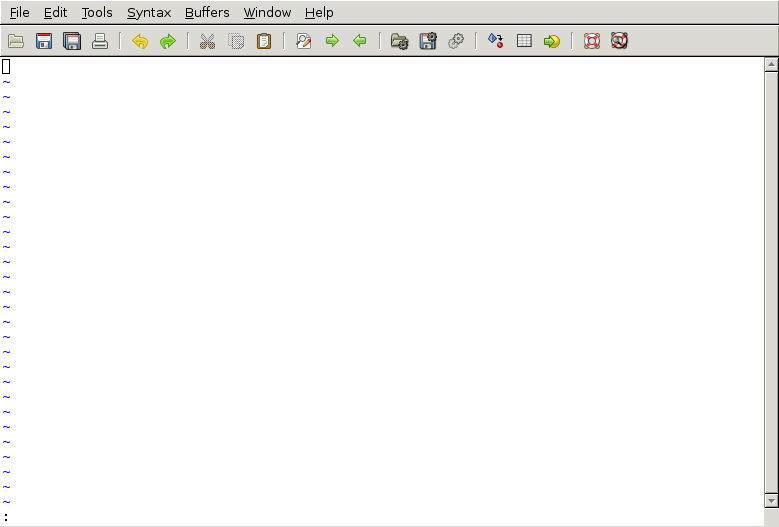
\includegraphics[width=\linewidth]{vim-new.png}
  \caption{Nouveau fichier vide.}
  \label{fig:vim-new}
\end{figure}

Commençons par entrer un commentaire dans d'entête du fichier pour y mentionner notre nom. Pour pouvoir entrer du texte appuyez sur \tti (le curseur devrait changer d'aspect) et entrez le commentaire ci-dessous\sidenote{Si vous ne savez pas trop ce que vous avez fait et que \vim vous affiche des trucs en rouge en bas à gauche au ne semble pas réagir comme il faut quand vous appuyez sur \tti, appuyez plusieurs fois sur \ttesc, ça devrait vous remettre au mode par défaut de \vim}.
\begin{listing}[H]

    \begin{minted}[bgcolor=bg, gobble=8]{vim}
        " VIM Configuration - Vincent Jousse
    \end{minted}
    \caption{Votre première ligne avec \vim.}
    \label{code:first-comment}
\end{listing}

Vous aurez remarqué que les commentaires en \emph{VimL} (le langage de configuration de \vim) commencent par un \Verb|"|. Appuyez ensuite sur \ttesc pour revenir au mode par défaut (le mode normal) de \vim. Et voilà le travail, cf figure \ref{fig:vim-first-comment}.

\begin{figure}%
  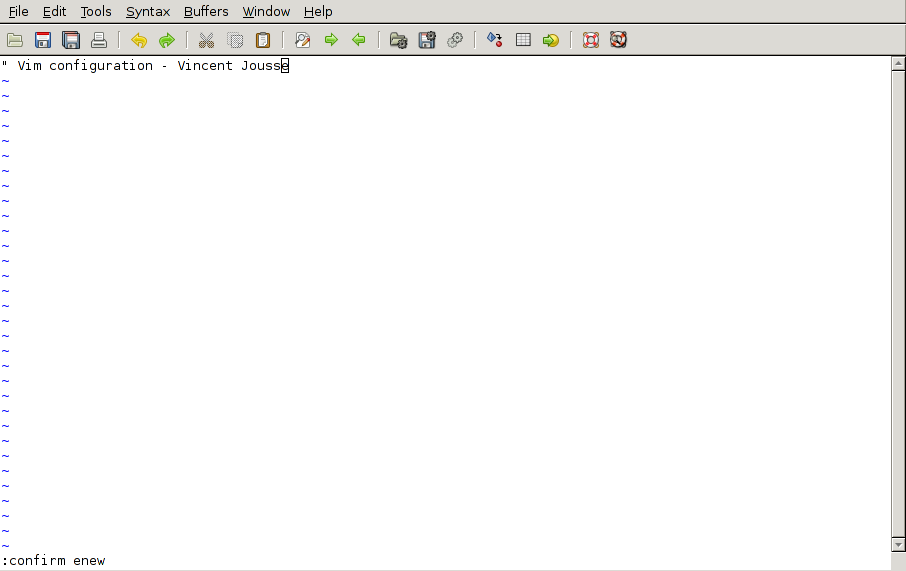
\includegraphics[width=\linewidth]{vim-first-comment.png}
  \caption{Mon premier commentaire.}
  \label{fig:vim-first-comment}
\end{figure}

Tout ça pour ça me direz vous, et vous avez bien raison. Mais tout cela a une logique que je vais vous expliquer. L'avantage de \vim est qu'il est généralement logique, quand vous avez compris la logique, tout vous semble limpide et tomber sous le sens.

Par défaut, \vim est lancé dans un mode que l'on appelle le mode ``Normal''. C'est à dire que ce mode n'est pas fait pour écrire du texte (ça, ça sera le mode ``Insert'') mais juste pour se déplacer et manipuler du texte. C'est la présence de ces 2 différents modes (il y en a d'autres mais ce n'est pas le sujet pour l'instant) qui fait toute la puissance de \vim. Il vous faudra un certain temps pour vous rendre compte de cette puissance par vous même, alors faites moi juste confiance pour l'instant.

Si vous vous demandez pourquoi ces modes, pourquoi on semble se compliquer la vie (on se la simplifie en fait) et en quel honneur, dans le mode par défaut, il n'est même pas possible d'insérer du texte, lisez attentivement la section qui suit.

\section{Les modes : d'où \vim tire sa puissance}

Je pense que nous serons tous à peu prêt d'accord sur le fait que si vous souhaitez apprendre à utiliser \vim, c'est pour gagner en efficacité pour la saisie/manipulation de texte/code. Pour gagner en efficacité lorsque l'on tape du code il n'y a pas 36 solutions, il n'y en a qu'une en fait : il faut bouger le moins possible les mains (voire pas du tout), et ne bouger que les doigts.

Pour ce faire bien sur, vous oubliez tout d'abord l'utilisation de la souris. En plus d'être lent, le mouvement clavier -> souris puis souris -> clavier est très mauvais pour vos articulations et les troubles musculosquelettiques en général\sidenote{Vous êtes peut-être jeune et n'avez pas encore eu ce type de soucis. Mais croyez moi, ça vient beaucoup plus vite qu'on ne le croit. Si vous passez votre journée sur un ordinateur, ne négligez pas ces facteurs, vous le regretterez un jour.}. D'après \emph{Wikipedia}, c'est le type de maladie professionnelle la plus courante à l'heure actuelle\sidenote{\url{https://fr.wikipedia.org/wiki/Troubles_musculosquelettiques}}.

Vous oubliez aussi le mouvement de votre main droite pour vous déplacer vers les touches directionnelles afin de bouger votre curseur. C'est une perte de temps et c'est totalement inutile avec \vim.

Qu'est-ce que vous avez le droit de faire dans le coup ? Pas grand chose, si ce n'est garder vos mains sur la position de repos comme le montre la figure \ref{fig:hand-position}. Vous trouverez d'ailleurs sur la plus part de claviers des marques sur les touches F et J, c'est pour vous donner un repère tactile d'où doivent se trouver vos indexes dans la position de repos.

\begin{figure}%
  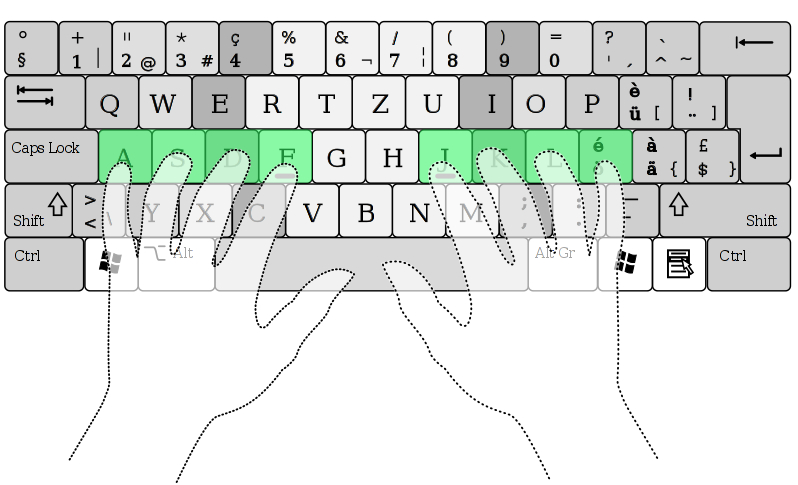
\includegraphics[width=\linewidth]{hand-position.png}
  \caption{Position de repos, clavier QWERTY. \emph{Illustration par Cy21 - CC-BY-SA-3.0 (\url{www.creativecommons.org/licenses/by-sa/3.0}) ou GFDL (\url{www.gnu.org/copyleft/fdl.html}), via Wikimedia Commons \url{http://commons.wikimedia.org/wiki/File:Typing-home-keys-hand-position.svg}}}
  \label{fig:hand-position}
\end{figure}

Ce parti pris (bouger le moins possible les mains du clavier) justifie à lui seul la présence d'un mode \emph{normal} et d'un mode \emph{insertion} dans \vim. En passant de l'un à l'autre, les touches sous vos doigts serviront tantôt à vous déplacer et à réaliser des opérations sur le texte\sidenote{C'est le mode \emph{normal}} (copier/coller, macros, \ldots), tantôt à sélectionner\sidenote{C'est le mode \emph{visuel}} et tantôt à insérer du texte\sidenote{C'est le mode \emph{insertion}}. Tout cela bien sur en évitant l'utilisation de combinaisons de touches du style \emph{Ctrl + touche} qui ne sont généralement pas bonnes pour vos doigts (\emph{Emacs} si tu nous lis, je te salue).

Par défaut, on passe du mode \emph{insertion} au mode \emph{normal} en appuyant sur la \ttesc, mais c'est une des premières choses que l'on changera : \ttesc est bien trop loin sur les claviers actuels. 

Pour passer du mode \emph{normal} au mode \emph{insertion}, on peut par exemple appuyer sur \tti On apprendra par la suite qu'il existe d'autre moyens de faire. Par exemple pour rentrer en mode insertion tout en créant une nouvelle ligne en dessous de la ligne courante (peut importe où se trouve votre curseur sur la ligne), on utilisera \tto en mode \emph{normal}.

\newthought{Si vous voulez pousser la démarche} jusqu'au bout, vous pouvez aussi vous procurer un clavier orthogonal \emph{TypeMatrix}\sidenote{\url{http://www.typematrix.com/}}. C'est ce que j'utilise personnellement, et mes doigts m'en remercient tous les jours.

\newpage
\section{La configuration par défaut : indispensable}

\newthought{Passons aux choses sérieuses}, c'est à dire comment rendre \vim un tant soit peu utilisable. Nous allons donc éditer le fichier de configuration par défaut \vimrc\sidenote{Ce fichier doit se trouver dans votre répertoire d'accueil. \emph{/home/votre\_user/.vimrc} sous Linux, \emph{/Users/votre\_user/.vimrc} sous Mac Os X ou plus généralement \emph{\textasciitilde{}/.vimrc}. Sous Windows vous pouvez créer un fichier nommé \emph{\_vimrc} qui doit se situer dans votre répertoire \emph{\%HOME\%} qui change en fonction de votre version de Windows. C'est généralement le répertoire jute "au dessus" de votre répertoire \emph{Mes Documents}. Plus d'infos sur Wikipedia \url{http://en.wikipedia.org/wiki/Home\_directory\#Default\_Home\_Directory\_per\_Operating\_System}} en y plaçant des valeurs que toute personne normalement constituée souhaiterait y voir figurer.

J'ai commenté chacune des lignes du fichier directement dans le code. Rien de sorcier ici, on se demande juste pourquoi tout cela n'est pas inclus par défaut.

\begin{listing}[H]
    \inputminted[bgcolor=bg, fontsize=\footnotesize]{vim}{../../vim-for-humans/firstconfig/vimrc}
    \caption{Une configuration par défaut sensée.}
    \label{code:first-config}
\end{listing}

J'ai mis en ligne ce fichier de configuration directement sur \emph{Github}. Vous pouvez le télécharger ou le copier directement à partir d'ici : \url{http://github.com/vjousse/vim-for-humans/fr/firstconfig/}. Il devrait aussi faire partie du package que vous avez téléchargé.

Vous devriez avoir un \vim qui ressemble à celui sur la figure \ref{fig:first-config}. Notez les numéros de ligne sur la gauche ainsi que la position du curseur en bas à droite.

\begin{figure}%
  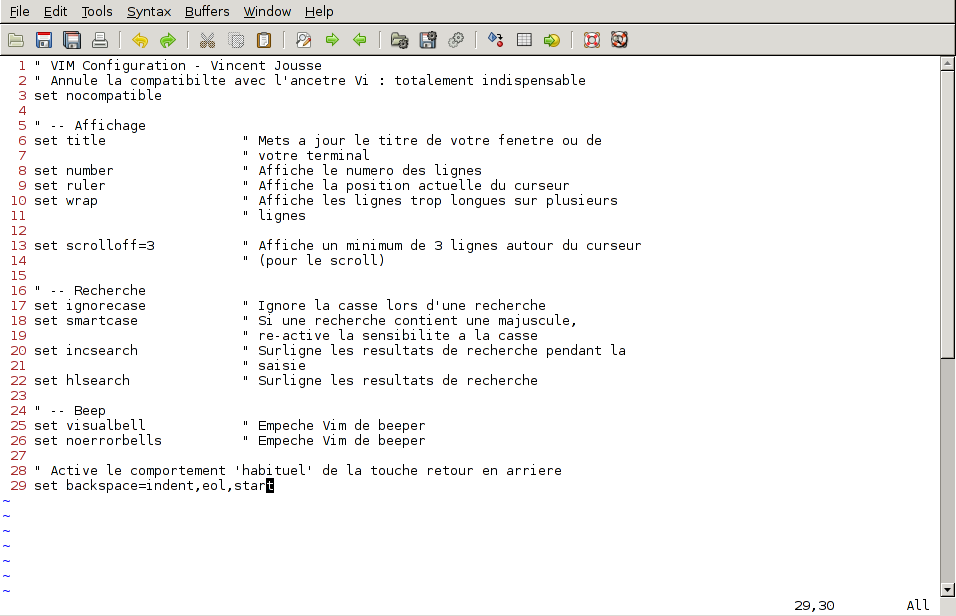
\includegraphics[width=\linewidth]{vim-first-config.png}
  \caption{\vim après votre première configuration.}
  \label{fig:first-config}
\end{figure}

Bon c'est bien beau tout ça mais ça manque un peu de couleurs. Au suivant !

\section{Que la couleur soit !}

\newthought{Tout d'abord} il faut commencer par activer la coloration syntaxique du code dans le fichier de configuration. Ajoutez ces lignes à là fin de votre fichier de configuration \vimrc.

\begin{listing}[H]
\begin{minted}[bgcolor=bg, fontsize=\footnotesize]{vim}
" Active la coloration syntaxique
syntax enable
" Active les comportements specifiques aux types de fichiers comme
" la syntaxe et l'indentation
filetype on
filetype plugin on
filetype indent on
\end{minted}
  \caption{Activation de la coloration syntaxique.}
  \label{lst:syntax-hl}
\end{listing}

Vous devriez avoir un \vim qui ressemble à celui de la figure \ref{fig:syntax-hl}\sidenote{Pour l'instant, le plus facile pour que les modifications apportées à votre \vimrc soient prisent en compte, c'est de le fermer et de le ré-ouvrir. Si vous voulez vraiment vous la jouer à la \vim de suite, en mode normal tapez \vimscmd{:so \textasciitilde/.vimrc}.

\vimscmd{:so} étant un raccourci pour \vimscmd{:source}.}. C'est une bonne première étape, passons maintenant à l'utilisation d'un thème.

\begin{figure}%
  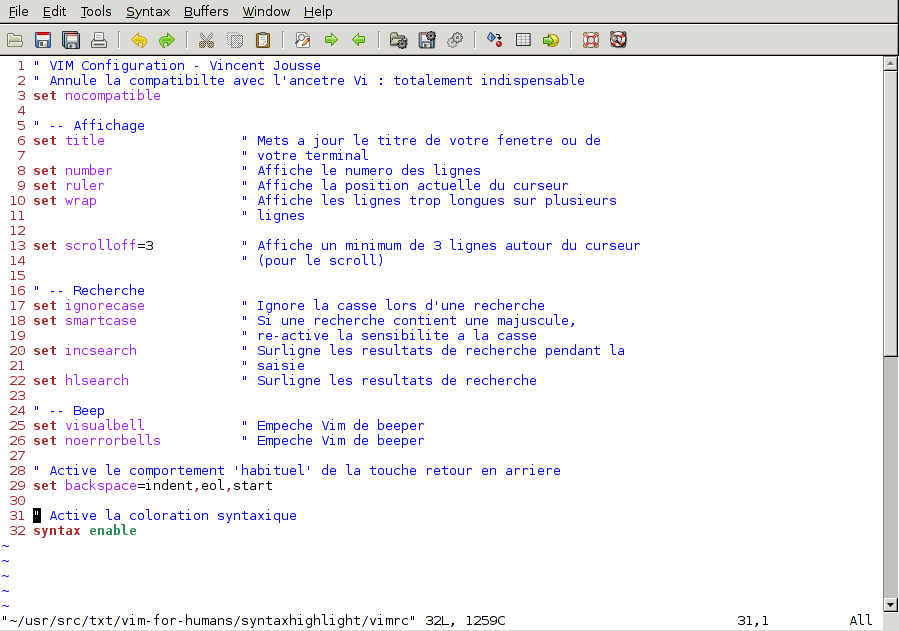
\includegraphics[width=\linewidth]{vim-syntax-hl.png}
  \caption{Coloration syntaxique par défaut.}
  \label{fig:syntax-hl}
\end{figure}

Les thèmes vont vous permettre de rendre votre \vim un peu moins austère en changeant généralement la couleur de fond ainsi que les couleurs par défaut pour le code. Comme je l'ai mentionné plus haut, nous allons utiliser le thème solarized \url{http://ethanschoonover.com/solarized} (avec fond clair ou foncé, ça dépendra de vous).

Pour l'installer, commencez tout d'abord par créer un répertoire nommé \Verb|.vim|\sidenote{Ce répertoire s'appelle \Verb|vimfiles| sous Windows. À chaque fois que je ferai référence au répertoire \Verb|.vim| ça sera en fait \Verb|vimfiles| pour les Windowsiens} au même endroit que votre \vimrc\sidenote{Dans votre répertoire utilisateur donc.}. Dans ce répertoire \Verb|.vim|, créez un sous-répertoire nommé \Verb|colors|. Téléchargez ensuite le fichier du thème Solarized \url{https://raw.github.com/altercation/vim-colors-solarized/master/colors/solarized.vim}\sidenote{ou copiez celui qui vous a été fourni avec le téléchargement de ce livre}(c'est le même fichier pour les deux versions du thème) et copiez le dans le répertoire \Verb|vim/colors/| fraichement créé. Activez ensuite le thème Solarized dans votre \vimrc comme le montre le code dans le listing \ref{lst:solarized}. Pour tester le thème clair, remplacez \Verb|dark| par \Verb|light| pour la valeur \Verb|background|.

\begin{listing}[H]
\begin{minted}[bgcolor=bg, fontsize=\footnotesize]{vim}
" Utilise la version sombre de Solarized
set background=dark
colorscheme solarized
\end{minted}
  \caption{Activation de la coloration syntaxique.}
  \label{lst:solarized}
\end{listing}

Les images \ref{fig:vim-solarized-dark} et \ref{fig:vim-solarized-light} vous donnent un aperçu des deux variantes (ma préférence allant à la variante sombre soit dit en passant).

\begin{figure}%
  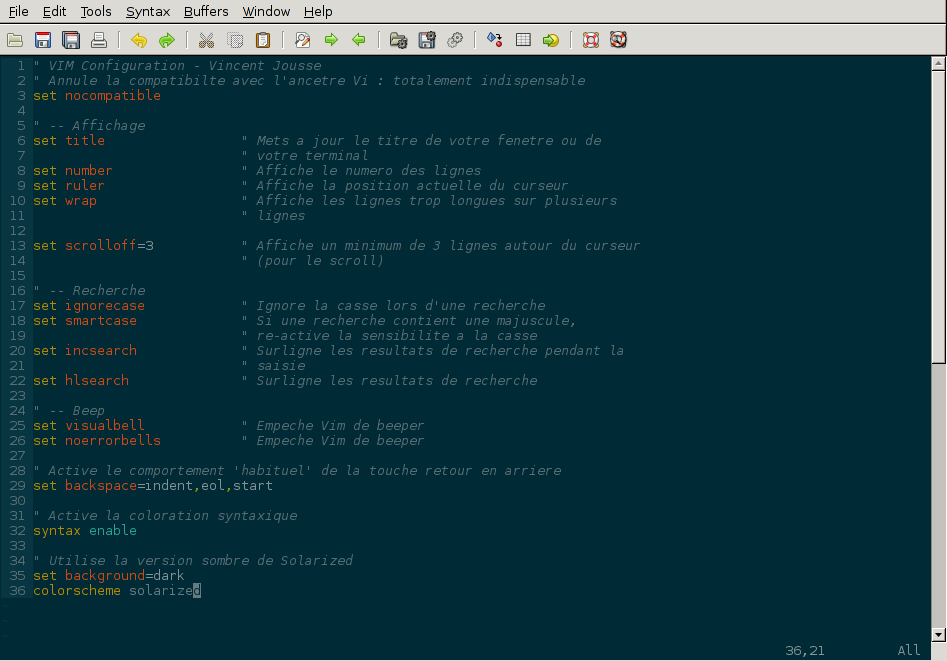
\includegraphics[width=\linewidth]{vim-solarized-dark.png}
  \caption{Le thème Solarized sombre.}
  \label{fig:vim-solarized-dark}
\end{figure}

\begin{figure}%
  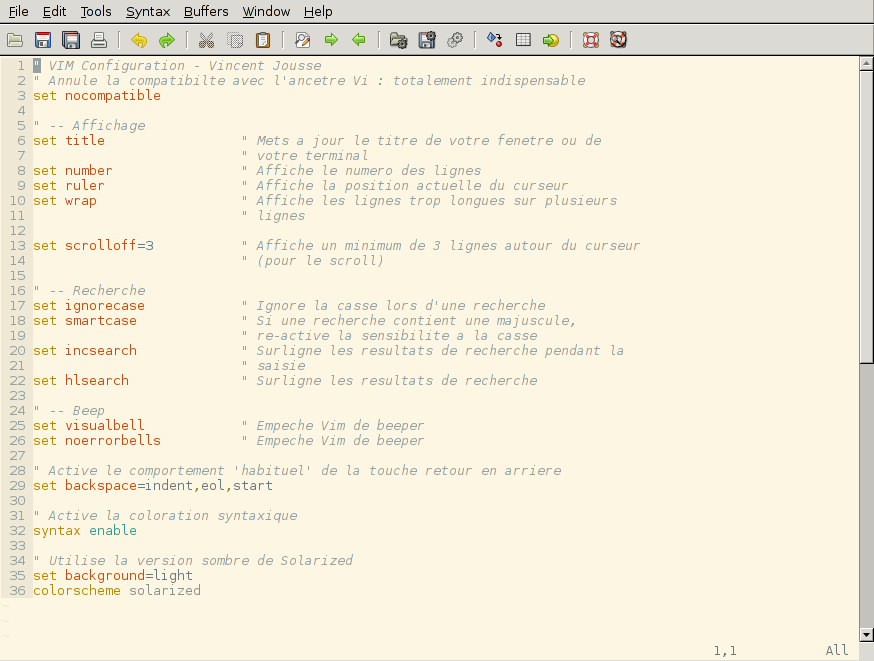
\includegraphics[width=\linewidth]{vim-solarized-light.png}
  \caption{Le thème solarized clair.}
  \label{fig:vim-solarized-light}
\end{figure}

\newthought{Un bonus} (si vous n'utilisez pas \vim directement dans votre terminal) serait de choisir une police de caractère qui vous convient un peu mieux, c'est bien sur facultatif mais bon, je présume que certains d'entre vous sont des esthètes aguerris.

Si vous êtes sous Mac Os X je vous conseille la police \Verb|Monaco| qui est plutôt sympathique. Rajoutez les lignes suivantes à votre \vimrc pour l'utiliser :

\begin{listing}[H]
\begin{minted}[bgcolor=bg, fontsize=\footnotesize]{vim}
set guifont=Monaco:h13
set antialias
\end{minted}
  \caption{Utilisation de la police Monaco sous Mac Os X.}
  \label{lst:monaco}
\end{listing}

Vous pouvez bien sur changer le \Verb|h13| par \Verb|h12| si vous voulez une police plus petite (ou par \Verb|h14| si vous en voulez une plus grande).

Sinon sous Linux j'utilise la police \Verb|DejaVu Sans Mono| que je trouve plutôt sympathique :

\begin{listing}[H]
\begin{minted}[bgcolor=bg, fontsize=\footnotesize]{vim}
set guifont=DejaVu\ Sans\ Mono\ 10
set antialias
\end{minted}
  \caption{Utilisation de la police DejaVuSansMono sous Linux.}
  \label{lst:dejavusansmono}
\end{listing}

Vous pouvez là aussi bien sur changer la taille de la police si vous le souhaitez. Pour avoir la liste des polices disponibles tapez on mode normal \vimcmd{:set guifont:*}.

Vous trouverez une version complète du fichier de configuration pour ce chapitre en ligne \url{https://github.com/vjousse/vim-for-humans/blob/master/syntaxhighlight/vimrc} ou avec les fichiers mis à disposition avec ce livre. Je ne m'attarderai pas plus sur les polices, c'est assez dépendant de votre système d'exploitation, et un peu moins de \vim dans le coup.


\section{L'explorateur de fichiers : notre premier plugin}

Nous y voilà, nous avons un \vim à peu près utilisable avec de jolies couleurs. Maintenant, il faudrait être capable d'ouvrir des fichiers autrement qu'en faisant \Verb|Fichier (File) -> Ouvrir (Open)|. Ça va être une bonne occasion pour installer notre premier plugin (ce n'est pas comme si nous avions d'autres choix de toute façon). Nous allons procéder ici en deux étapes, tout d'abord installer un gestionnaire de plugin pour éviter que ça devienne trop le bazaar dans vos plugins, puis installer ensuite le plugin qu'il nous faut pour explorer un répertoire de fichiers.

\subsection{Gestionnaire de plugins: Pathogen}

Pathogen\sidenote{\url{https://github.com/tpope/vim-pathogen/}} est typique du plugin que vous découvrez après avoir commencé à configurer votre \vim et qui génère ce type de réaction : "Ah si j'avais su j'aurais directement commencé avec". Ça tombe bien, c'est ce que nous allons faire.

Tout d'abord petite explication de comment on installe et configure des plugins dans \vim. Ils s'installent en copiant les fichiers adéquats (la plus part du temps avec une extension en \emph{*.vim}) dans des sous répertoires de votre répertoire de configuration \emph{.vim}. On a déjà d'ailleurs commencé à y créer un sous-répertoire \Verb|colors| qui contient notre "plugin" de coloration Solarized.

Le problème avec cette approche c'est que les différents plugins ne sont pas isolés (vous allez devoir copier leurs fichiers dans les différents sous-répertoires) et que vous allez donc vous retrouver avec des fichiers un peu partout sans savoir à qui ils appartiennent. Autant vous dire qu'une fois que vous voulez désinstaller ou mettre à jour un plugin, c'est vite l'enfer pour savoir quels sont ses fichiers.

C'est la que pathogen arrive à la rescousse, il va vous permettre d'installer chaque plugin dans un sous répertoire rien que pour lui. La figure \ref{fig:pathogen-tree} vous donne un exemple de répertoire \Verb|.vim| avant et après l'utilisation de pathogen. Certes la version avec pathogen contient plus de sous répertoires, mais croyez moi sur parole, ce rangement va vous éviter bien des ennuis par la suite\sidenote{Et vous pourrez au passage très facilement utiliser \emph{git} pour gérer chacun de vos plugins comme des submodules, ce qu'il est impossible de réaliser sinon.}.

\begin{figure}%
  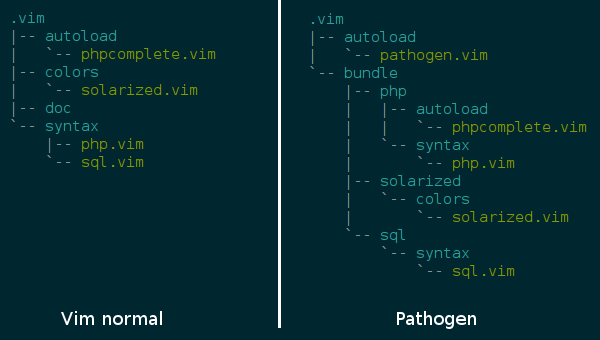
\includegraphics[width=\linewidth]{pathogen-tree.png}
  \caption{\emph{.vim} avant et après Pathogen.}
  \label{fig:pathogen-tree}
\end{figure}

Commençons par installer pathogen. Créez un répertoire nommé \Verb|autoload| dans votre répertoire \Verb|.vim| et copiez y \Verb|pathogen.vim| que vous pouvez télécharger ici : \url{https://raw.github.com/tpope/vim-pathogen/master/autoload/pathogen.vim} (ou qui vous a été fourni avec ce PDF). Pour les utilisateurs Unix, le listing \ref{code:pathogen-install} explique comment l'installer\sidenote{Si vous n'avez pas \Verb|{\footnotesize curl}| vous pouvez aussi utiliser \scmd{wget -O -}}.

\begin{listing}[H]
\begin{minted}[bgcolor=bg, fontsize=\footnotesize]{sh}
# Creation du repertoire autoload
mkdir -p ~/.vim/autoload 

# Telechargement et installation de pathogen
curl -so ~/.vim/autoload/pathogen.vim \
    https://raw.github.com/tpope/vim-pathogen/master/autoload/pathogen.vim
\end{minted}
  \caption{Installation de pathogen.}
  \label{code:pathogen-install}
\end{listing}

Nous installerons ensuite nos plugins directement dans le répertoire \Verb|.vim/bundle| que vous allez vous empresser de créer, cf. le listing \ref{code:pathogen-bundle}.

\begin{listing}[H]
\begin{minted}[bgcolor=bg, fontsize=\footnotesize]{sh}
# Creation du repertoire bundle
mkdir -p ~/.vim/bundle
\end{minted}
  \caption{Création du répertoire d'installation des plugins.}
  \label{code:pathogen-bundle}
\end{listing}

Il ne vous reste plus qu'à activer pathogen dans votre \vimrc et le tour est joué. Nous placerons le code listé dans 
\ref{code:pathogen} au début du fichier \vimrc, directement après la ligne \Verb|set nocompatible|.

\begin{listing}[H]

\begin{minted}[bgcolor=bg]{vim}
" Activation de pathogen
call pathogen#infect()
\end{minted}
\caption{Activation du plugin pathogen.}
\label{code:pathogen}
\end{listing}

Puisque charité bien ordonnée commence par soit même, nous allons ranger notre petit plugin solarized en utilisant pathogen. Il nous suffit de créer un répertoire \Verb|solarized| dans notre répertoire \Verb|bundle| fraichement créé\sidenote{Vous pouvez l'appeler comme vous le souhaitez, tout sous-répertoire du répertoire \Verb|{\footnotesize bundle}| sera considéré comme un répertoire de plugin.}. Nous déplaçons ensuite le répertoire \Verb|colors| dans le répertoire \Verb|solarized| cf. le listing \ref{code:solarized-bundle}.

\begin{listing}[H]
\begin{minted}[bgcolor=bg, fontsize=\footnotesize]{sh}
# Creation du repertoire pour solarized
mkdir ~/.vim/bundle/solarized
# Et hop un peu de rangement
mv ~/.vim/colors ~/.vim/bundle/solarized
\end{minted}
  \caption{Utilisation de solarized via pathogen.}
  \label{code:solarized-bundle}
\end{listing}

Voilà notre \vim est presque près pour le grand bain. Il vous reste une petite étape à franchir : disposer d'un moyen pratique pour explorer les fichiers d'un projet, c'est ici que \emph{The NERD Tree} entre en lisse.

\subsection{Explorateur de fichiers : The NERD Tree}

The NERD Tree est un plugin permettant d'afficher visuellement une arborescence de fichiers directement dans la partie gauche (par défaut) dans votre \vim à la \emph{TextMate}, \emph{Sublime Text} ou encore \emph{Eclipse/Netbeans}. Ce plugin n'est pas essentiel si vous souhaitez tout contrôler au clavier (je ne l'utilise plus moi même), mais est assez pratique lorsque l'on débute avec \vim.

L'alternative que nous verrons plus tard au chapitre \TODO est d'utiliser le plugin \emph{Ctrl-p} pour trouver des fichiers et les plugins \emph{LustyExplorer} et \emph{LustyJuggler} pour naviguer entre les fichiers. En effet, devoir visualiser l'arborescence pour trouver un fichier est toujours plus lent que de trouver le fichier à partir de son nom par exemple. The NERD Tree vous permettra donc d'obtenir un \vim se comportant comme un éditeur classique avec un explorateur de fichiers sur lequel vous pourrez cliquer.

Nous allons tout d'abord préparer pathogen pour installer les différents fichiers de \emph{The NERD Tree}.

\begin{listing}[H]
\begin{minted}[bgcolor=bg, fontsize=\footnotesize]{sh}
# Creation du repertoire pour The NERD Tree
mkdir ~/.vim/bundle/nerdtree
\end{minted}
  \caption{Création du répertoire pour The NERD Tree.}
  \label{code:nerdtree-bundle}
\end{listing}

Téléchargez ensuite le dernier \emph{.zip} disponible sur la page du plugin \url{http://www.vim.org/scripts/script.php?script_id=1658}. À l'heure où j'écris ces lignes la dernière version disponible est la version 4.2.0 disponible en téléchargement à cette adresse\sidenote{C'est la version que vous trouverez dans les fichiers mis à disposition avec ce PDF} : \url{http://www.vim.org/scripts/download_script.php?src_id=17123}.

Ouvrez le fichier zip et placez son contenu dans le répertoire \Verb|~/.vim/bundle/nerdtree| que nous venons de créer. Vous devriez avoir une arborescence ressemblant à celle ci-dessous pour votre répertoire \Verb|nerdtree| :

\begin{verbatim}
nerdtree
|-- doc
|   `-- NERD_tree.txt
|-- nerdtree_plugin
|   |-- exec_menuitem.vim
|   `-- fs_menu.vim
|-- plugin
|   `-- NERD_tree.vim
`-- syntax
    `-- nerdtree.vim
\end{verbatim}

Il va ensuite falloir activer le plugin. Vous pouvez le faire manuellement en tapant \vimcmd{:NERDTree} en mode normal. Si vous préférez activer \emph{The NERD Tree} à chaque fois que vous ouvrez votre \vim, ajoutez ces lignes dans votre \vimrc:

\begin{listing}[H]
\begin{minted}[bgcolor=bg]{vim}
" Activation de NERDTree au lancement de vim
autocmd vimenter * NERDTree
\end{minted}
\caption{Activation de NERDTree au lancement de \vim.}
\label{code:pathogen}
\end{listing}

Rien de particulier ensuite, \emph{The NERD Tree} vous affiche l'arborescence du répertoire où vous avez lancé \vim, comme vous le montre la figure \ref{fig:vim-nerdtree}. Vous pouvez utiliser la souris et/ou le clavier pour vous déplacer. 

Vous pouvez aussi effectuer des commandes (créer, copier des fichiers) en appuyant sur \ttm lorsque vous êtes dans \emph{The NERD Tree}. Pour passer de la fenêtre de \emph{NERD Tree} à la fenêtre d'édition de votre fichier au clavier, appuyez sur \hlred{Ctrl + w + w}\sidenote{La touche \hlred{\emph{Control}} (Ctrl) et tout en la laissant appuyée, deux fois \hlred{w}.}. Ce raccourci clavier sera d'ailleurs toujours valable pour naviguer entre vos différentes fenêtres \vim (il n'est pas spécifique à \emph{The NERD Tree}).

\begin{figure}%
  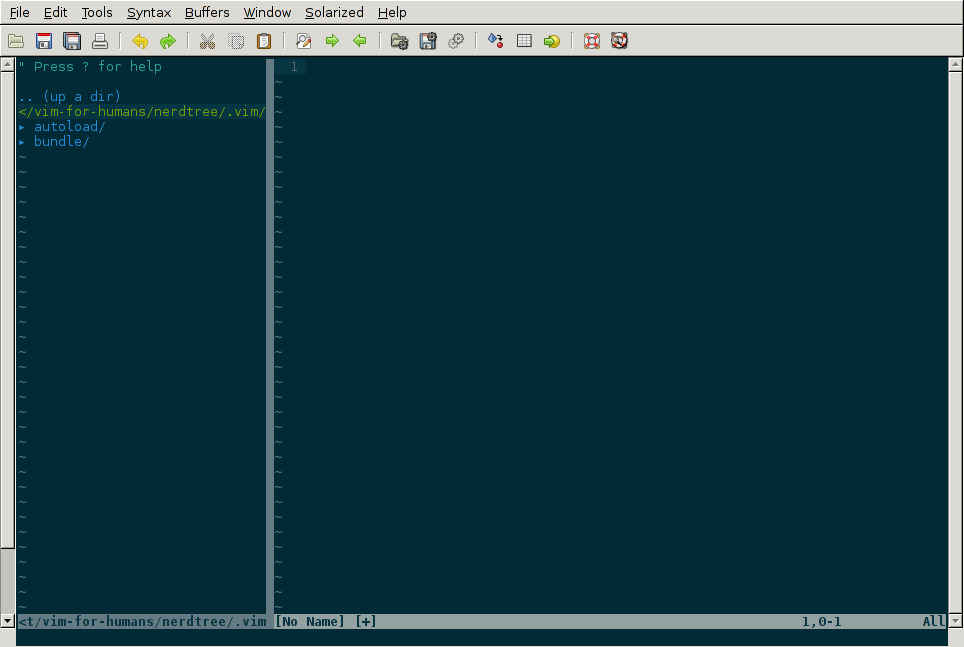
\includegraphics[width=\linewidth]{vim-nerdtree.png}
  \caption{\emph{.vim} avec \emph{The NERD Tree} d'activé.}
  \label{fig:vim-nerdtree}
\end{figure}


\chapter{L'outil de manipulation de texte rêvé}

Alors oui, pour ceux qui se demandent, je fais des rêves bizarres, mais bon chacun a ses petites tares cachées. Et rêver d'un outil qui améliore ma vie quotidienne en tant que codeur (ou écrivain, ou formateur, ou \ldots) n'est pas si étrange que ça.

Ce qui fait et fera encore le succès de \vim est sa capacité à \textbf{faciliter les manipulations de texte}. Certes il va vous proposer des fonctionnalités propres à chaque tâche que vous effectuerez \footnote{Souvent par l'intermédiaire de plugins.} comme la validation syntaxique de code, la correction orthographique, \ldots Mais à la fin, c'est toujours à écrire/corriger/manipuler/se déplacer dans du texte que vous passerez la majeure partie de votre temps. 

C'est là que l'approche de \vim est différente d'IDE comme Eclipse / Netbeans / PhpStorm et consorts. Là où ces IDE vont mettre l'accent sur les particularités de votre langage de programmation tout en vous fournissant des capacités de manipulation de texte basiques, \vim adopte l'approche opposée : vous serez \textbf{très efficace} à manipuler/écrire du texte quel que soit le texte et vous pourrez enrichir \vim avec des fonctionnalités propres à votre langage de programmation via des plugins.

Nous allons donc voir dans ce chapitre comment utiliser \vim à bon escient (vous allez commencer à oublier votre souris) et quelle est la logique derrière tous ces enchaînements de commandes qui paraissent barbares au non-initié. Vous devriez pouvoir, à la fin de ce chapitre, \textbf{vous passer de votre souris} pour éditer/manipuler le contenu d'un fichier\footnote{En tout cas, vous devriez vous forcer à le faire en apprenant \vim, ce n'est pas si dur que ça, et c'est ce qui fait la différence entre \vim et les autres : le tout clavier.}.

\section{Se déplacer par l'exemple : Essayer de copier / coller}\label{sec:se-deplacer}


Nous avons déjà vu dans la section «\nameref{sec:modeinsertion}» comment passer du mode insertion (pour saisir du texte) au mode normal (\emph{a priori} pour l'instant, vous ne savez pas trop à quoi sert ce mode). En appuyant sur \tti votre curseur passe en mode insertion (lorsque vous êtes en mode normal) et en appuyant sur \ttesc il repasse dans le mode normal. Bon bah on est bien Tintin. Et maintenant ? 

\subsection{Préambule}

Nous allons apprendre notre première manipulation de texte : le copier / coller. J'en vois certains d'entre vous se dire que ça ne sert à rien, car vous savez déjà le faire. Vous passez en mode insertion, vous prenez votre souris (ou vous vous déplacez avec les flèches directionnelles tout en appuyant sur \ttshift) pour sélectionner du texte et vous allez dans le \Verb|menu Édition| puis \Verb|Copier|. Et ensuite \Verb|menu Édition| puis \Verb|Coller|. Bah tiens, essayez pour voir.

Si vous avez suivi la section «\nameref{sec:modes}» traitant de la position idéale pour vos mains, vous savez que vous avez fait une ou plusieurs choses que vous devriez vous interdire :


\begin{itemize}
    \item Vous avez utilisé votre souris
    \item Vous avez déplacé grandement votre main droite de sa position de repos, pour aller atteindre les flèches directionnelles qui sont très mal placées sur un clavier
\end{itemize}


Alors certes ce n'est pas grave en soi, mais c'est \textbf{inefficace} (se servir de la souris ou déplacer votre main droite vers les touches directionnelles est très lent) et \textbf{nuisible} pour vos petites mains. Ceci est votre dernière chance : si vous n'êtes pas prêt à vous forcer à ne pas le faire, \textbf{\vim n'est pas fait pour vous}. \vim est parfait pour ne pas utiliser la souris et pour ne pas bouger vos mains (ou presque). Ne pas se forcer à le faire, c'est ne pas tirer partie de tout le potentiel de \vim, et à un moment ou un autre, \textbf{vous le quitterez pour un éditeur} qui aura été pensé pour être utilisé à la souris. Alors, on continue ?

\subsection{Se passer de la souris}

Si vous lisez ces lignes c'est que vous avez répondu « oui », allons-y gaiement alors ! Nous allons tout d'abord commencer par nous passer de la souris. La prochaine étape sera de se passer des touches directionnelles, mais chaque chose en son temps.


\newthought{Pour réaliser un copier/coller} avec \vim tout se passe en mode « normal ». Pour savoir dans quel mode vous vous trouvez, vous avez juste à regarder en bas à gauche de votre \vim. La figure \ref{fig:insert} vous montre \vim en mode « insertion » par exemple. Lorsque rien n'est marqué en bas à gauche, c'est que vous êtes en mode normal. Pour sortir d'un mode afin de retourner au mode normal, il suffit d'appuyer sur \ttesc\footnote{Si vous vous demandez pourquoi je vous dis d'arrêter d'utiliser la souris et/ou les touches directionnelles, mais que je ne dis rien sur le fait qu'il faille se torturer la main pour atteindre \ttesc, c'est que vous êtes sur la bonne voie. Je vous explique le comment du pourquoi dans «\nameref{sec:esc}».}.

\begin{figure}%
  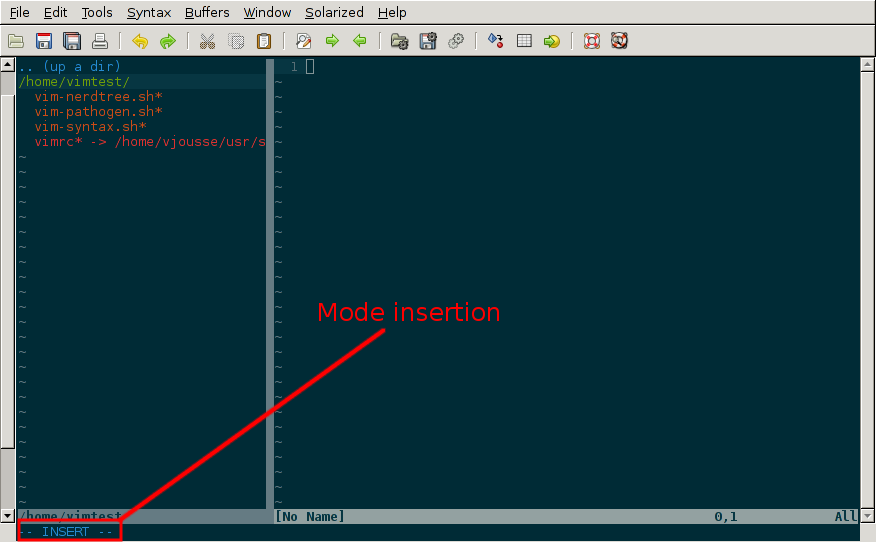
\includegraphics[width=\linewidth]{vim-insert.png}
  \caption{\vim en mode insertion.}
  \label{fig:insert}
\end{figure}

Admettons donc que vous êtes en mode « normal » et que vous avez un peu de texte de saisi dans votre \vim. Par exemple, cette chouette citation de Mark Twain : « Ils ne savaient que c'était impossible, alors ils l'ont fait. ». Votre \vim devrait ressembler à celui de la figure \ref{fig:vim-twain}\footnote{Notez l'absence d'affichage d'un quelconque mode en bas à gauche.}.

\begin{figure}%
  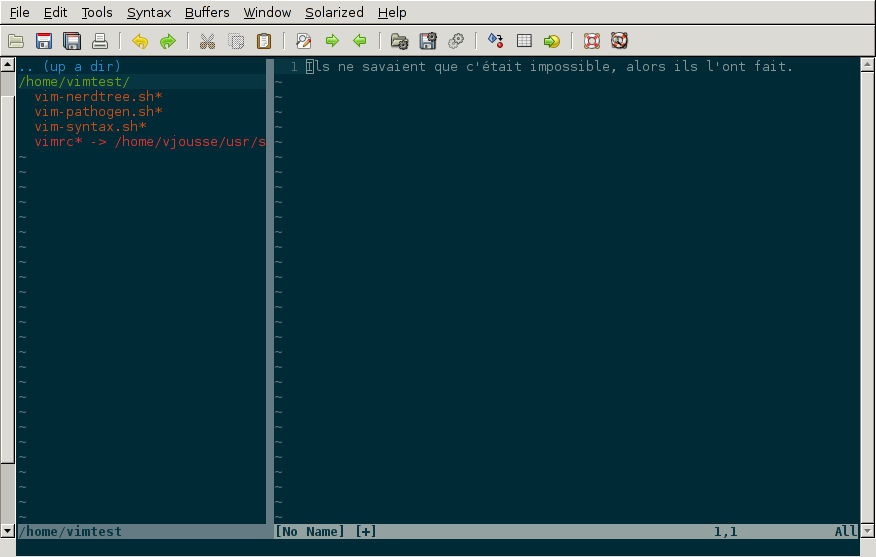
\includegraphics[width=\linewidth]{vim-twain.png}
  \caption{\vim prêt pour le copier/coller.}
  \label{fig:vim-twain}
\end{figure}

La façon la plus naturelle\footnote{Mais pas la plus efficace, nous verrons cela un peu plus loin.} de copier/coller le mot « impossible » va être de se déplacer sur la première lettre du mot avec les touches directionnelles, d'appuyer sur \ttv (pour passer en mode « visuel »), de se déplacer sur la dernière lettre (vous devriez avoir le mot sélectionné, en surbrillance) puis d'appuyer sur \tty\footnote{La touche \ty étant utilisée comme raccourci du mot \emph{yank} en anglais.}. Vous avez copié votre premier mot.

Déplacez vous ensuite à la fin de la phrase (toujours en mode « normal ») puis appuyez sur \ttp\footnote{Raccourci du mot \emph{paste} cette fois ci.}. Le mot devrait avoir été collé à la fin, et vous devriez avoir le même rendu que la figure \ref{fig:vim-paste}.

\begin{figure}%
  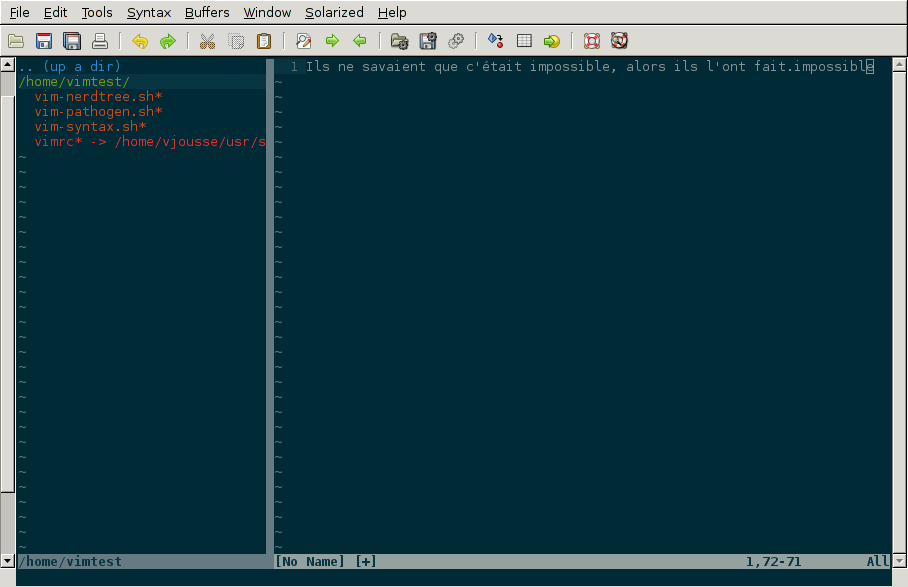
\includegraphics[width=\linewidth]{vim-paste.png}
  \caption{\vim après le copier/coller.}
  \label{fig:vim-paste}
\end{figure}

On se rend donc compte ici que \vim se sert de l'astuce des modes (et notamment du mode « normal » pour les déplacements) afin de ne pas avoir à se servir de la souris.
À partir du moment où vous aurez pris l'habitude de passer rapidement d'un mode à l'autre (et pour cela se passer de \ttesc va devenir indispensable), utiliser la souris vous apparaîtra comme une perte de temps, mais pour cela il va falloir pratiquer un peu bien sûr.


\section{Se passer des touches directionnelles}\label{sec:se-passer-touches-dir}

Nous y voilà. Encore plus que de se priver de la souris, se priver des touches directionnelles est la chose à faire si l'on veut utiliser \vim, pour de vrai. \vim va vous permettre de faire tout plus rapidement et plus intuitivement à la seule condition de le faire sans les touches directionnelles.
Cela va vous permettre comme je l'ai déjà dit de ne pas bouger votre main certes, mais ça va aussi vous forcer à passer en mode « normal » pour réaliser vos déplacements et vos mouvements de texte. Il n'y a qu'à ce moment là\footnote{Un peu douloureux au début il est vrai.} que vous commencerez à vraiment tirer parti de \vim.

Pour cette section, je vais vous expliquer comment vous déplacer sans utiliser les touches directionnelles. Puis, une fois que vous aurez une vague idée de comment faire, je vous donnerai le code à mettre dans votre \vimrc pour désactiver les touches directionnelles complètement. Car oui, il n'y a que comme ça que vous y arriverez (en tout cas il n'y a que comme ça que j'y suis arrivé).


\subsection{Se déplacer sans les touches directionnelles}

En mode normal, 4 touches vont vous permettre de déplacer le curseur d'un caractère :
\begin{itemize}
    \item \tth pour aller \textbf{à gauche}
    \item \ttj pour aller \textbf{en bas}
    \item \ttk pour aller \textbf{en haut}
    \item \ttl pour aller \textbf{à droite}
\end{itemize}

\begin{figure}%
  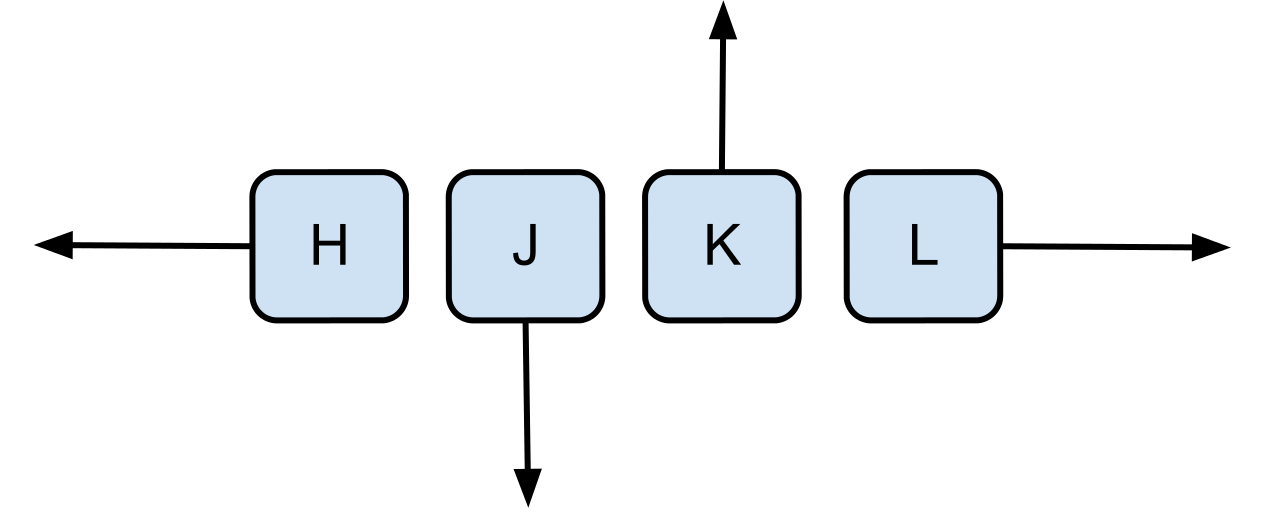
\includegraphics[width=\linewidth]{hjkl.png}
  \caption{Les « touches directionnelles » de \vim en mode normal.}
  \label{fig:vim-hjkl}
\end{figure}

Vous pouvez remarquer que ces touches sont placées sur la rangée de repos de manière à déplacer vos doigts le moins possible. En essayant de placer vos doigts pour atteindre ces lettres vous devriez vous rendre compte que l'index a deux déplacements (gauche et bas) alors que l'auriculaire n'en a pas. Vous verrez qu'on s'y fait assez rapidement et que l'index étant plus fort que l'auriculaire, ça tombe plutôt bien\footnote{Vous trouverez le clavier sur lequel \emph{Vi} a été conçu dan la section «\nameref{sec:esc}», vous comprendrez ainsi le pourquoi du comment.}.

À noter qu'à force, on se sert de moins en moins des déplacements gauche/droite d'un caractère. On va leur préférer les déplacements de mot en mot, de paragraphe en paragraphe ou les déplacements grâce à des recherches. Quelques exemples de déplacements "rapides" que j'utilise :

\bigskip

\begin{tabular}[H]{|c|c|}
  \hline
  Touche & Déplacement \\
  \hline
  \te & \textbf{à la fin du mot courant} \\
  \tb & \textbf{au début du mot courant} \\
  \tw & \textbf{au début du mot suivant} \\
  \that & \textbf{au premier caractère non blanc de la ligne} \\
  \tdollar & \textbf{à la fin de la ligne} \\
  \tzero & \textbf{au début de la ligne} \\
  \hline
\end{tabular}

\bigskip

Vous avez ici le minimum pour vous déplacer en mode normal. Il existe aussi des commandes vous permettant de vous déplacer puis de rentrer en mode insertion directement, elles sont très pratiques car elles vont vous permettre d'économiser quelques touches. En voici quelques unes que j'utilise à peu près tout le temps :

\bigskip
\begin{tabular}[H]{|c|c|}
  \hline
  Touche & Action \\
  \hline
  \ti & se place en mode insertion \textbf{avant l'emplacement du curseur} \\
  \ta & se place en mode insertion \textbf{après l'emplacement du curseur} \\
  \tI & se place en mode insertion \textbf{au début de la ligne} \\
  \tA & se place en mode insertion \textbf{à la fin de la ligne} \\
  \kto & insère une nouvelle ligne \textbf{en dessous de la ligne courante} \\
  \tO & insère une nouvelle ligne \textbf{au dessus de la ligne courante} \\
  \tr & \textbf{remplace les caractères} sous le curseur \\
  \hline
\end{tabular}
\bigskip

Arrêtons-nous un peu là dessus. Au risque d'insister lourdement, mais la clé de l'utilisation de \vim vient de ce que nous venons de voir dans ce chapitre, ni plus, ni moins. Il y a une chose que vous avez à vous forcer à faire, c'est \textbf{d'utiliser les touches hjkl} pour les déplacements. Si vous y arrivez, tout le reste vous l'apprendrez au fur et à mesure.

Vous trouverez des sites entiers vous détaillant les différentes commandes possibles, les différentes combinaisons, j'en passe et des meilleures. Vous les apprendrez puis les oublierez (ou pas, en fonction de si elles vous sont vraiment utiles). Si vous avez un seul effort à faire c'est celui de se passer des touches directionnelles et donc de vous forcer à utiliser le mode normal. Le reste tombera sous le sens.

Voici l'ultime configuration qu'il vous faudra mettre dans votre \vimrc pour atteindre le Saint Graal : désactiver les touches directionnelles.

\begin{listing}[H]

    \begin{minted}[bgcolor=bg, gobble=8]{vim}
        " Desactiver les touches directionnelles
        map <up> <nop>
        map <down> <nop>
        map <left> <nop>
        map <right> <nop>
        imap <up> <nop>
        imap <down> <nop>
        imap <left> <nop>
        imap <right> <nop>
    \end{minted}
    \caption{Désactiver les touches directionnelles.}
    \label{code:touches-directionnelles}
\end{listing}

Nous y voilà. Croyez-moi, vous allez souffrir un peu au début. Pour moi, ça n'a pas du durer plus de 2 jours. Ensuite vous aurez oublié. Si vous n'êtes pas prêt à galérer un peu pendant deux jours pour améliorer votre efficacité à vie, que faites vous ici !

Je ne vous donnerai pas beaucoup plus d'autres détails sur toutes les touches possibles et imaginables pour vous déplacer, d'autres ressources le font déjà bien mieux que moi. Je vais en revanche vous apprendre dans \nameref{sec:combine-move} comment les utiliser à bon escient.

On peut notamment citer le livre gratuit "A byte of \vim" traduit en français et disponible à l'adresse suivante : \url{http://www.swaroopch.org/notes/Vim_fr:Table_des_Mati\%C3\%A8res}.

Ou encore l'infographie de la figure \ref{fig:vim-cheat-sheet}\footnote{Téléchargeable sur \url{http://www.nathael.org/}} qui donne un aperçu des différents mouvements pour chacune des touches d'un clavier français.

\begin{figure}%
  \includegraphics[width=\linewidth]{vi-vim-cheat-sheet.png}
  \caption{Les touches \vim.}
  \label{fig:vim-cheat-sheet}
\end{figure}

N'oubliez pas que le but ici est de gagner en rapidité en ne bougeant quasi plus ses mains de la rangée de repos, et en utilisant le plus possible le « mode normal ». Au boulot !

\section{Se passer de la touche Échap}\label{sec:esc}

Utiliser \ttesc pour sortir du mode « insertion » semble être une hérésie tellement elle est difficilement accessible. Il faut déplacer entièrement la main gauche pour y accéder ou alors se torturer le petit doigt.

Pour comprendre pourquoi \ttesc est utilisée par défaut, il faut faire un bon de quelques années en arrière, pour se retrouver en face du clavier sur lequel \emph{Vi} a été développé. Vous pouvez voir sur la photo \ref{fig:vim-keyboard} que \ttesc était très facilement accessible. Vous pouvez aussi noter l'emplacement des touches directionnelles. Malheureusement depuis, cela a bien changé.

\begin{figure}%
  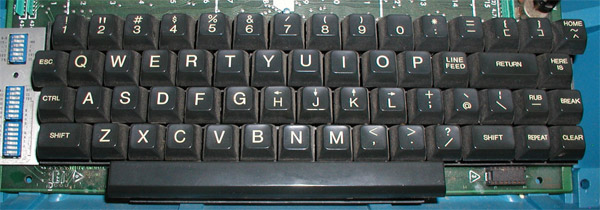
\includegraphics[width=\linewidth]{lsi-adm3a-full-keyboard.jpg}
  \caption{Le clavier sur lequel \emph{Vi} a été réalisé.}
  \label{fig:vim-keyboard}
\end{figure}

L'étape ultime (après avoir réussi à se passer des touches directionnelles) est donc de rapprocher \ttesc de vos petits doigts. Il y a plusieurs solutions pour cela, mais celle que je vous recommande si vous avez un clavier avec une disposition française est la suivante (dans votre \vimrc) :

\begin{listing}[H]

    \begin{minted}[bgcolor=bg, gobble=8]{vim}
        " Les ; sons rarement utilise l'un a la suite de l'autre
        :imap ;; <Esc>
    \end{minted}
    \caption{Taper deux fois sur \hlred{;} pour quitter le mode normal.}
    \label{code:avoid-esc}
\end{listing}

Lorsque vous êtes en mode insertion, il vous suffit d'appuyer deux fois sur \ttsemicolon pour retourner au mode normal. \ttsemicolon ne vous demande pas de bouger votre main de la rangée de repos et on l'utilise rarement deux fois de suite (et si c'est le cas, il suffit d'attendre un peu avant de taper le deuxième \tsemicolon), c'est donc le parfait candidat.

Voici d'autres solutions possibles (cf \url{http://vim.wikia.com/wiki/Avoid_the_escape_key}):

\begin{listing}[H]
    \begin{minted}[bgcolor=bg, gobble=8]{vim}

        :imap jj <Esc>

        :imap jk <Esc>

        :imap ii <Esc>

        :imap ` <Esc>

        " Shift-Espace (peut ne pas marcher sur votre systeme).
        :imap <S-Space> <Esc>

        " Sous Linux avec gvim Vim en console, vous pouvez utiliser Alt-Space.
        :imap <M-Space> <Esc>
    \end{minted}
    \caption{D'autres combinaisons de touches possibles pour quitter le mode normal.}
    \label{code:avoid-esc-alt}
\end{listing}

\section{Combiner des touches/déplacements}
\label{sec:combine-move}

Maintenant que nous savons nous déplacer en mode normal, il est temps de voir comment réaliser d'autres opérations. Nous avons déjà vu le copier/coller au chapitre \nameref{sec:se-deplacer}, nous allons maintenant voir comment supprimer/éditer plus facilement.

Dans \nameref{sec:se-passer-touches-dir} nous avons vu qu'il suffisait d'utiliser \ttw pour se déplacer au début du mot suivant. Nous allons essayer de combiner cela avec quelques nouvelles touches du mode normal :

\begin{itemize}
    \item \ttd est utilisée pour « supprimer »
    \item \ttc est utilisée pour « supprimer et passer en mode insertion »
\end{itemize}

À noter que ce qui est supprimé est placé dans le presse-papier en même temps (le « supprimer » se comporte par défaut comme un « couper »).

La particularité de ces touches, c'est qu'elles attendent ensuite un « ordre de déplacement » pour savoir quoi supprimer. Il va donc falloir les combiner avec les déplacements que nous avons déjà vus dans \nameref{sec:se-passer-touches-dir}.

Cela donnera par exemple :


\bigskip
\begin{tabular}[H]{|c|c|}
  \hline
  Action & Résultat \\
  \hline
  \ttd puis \ttw & supprime les caractères jusqu'au prochain mot \\
  \ttc puis \ttw & supprime les caractères jusqu'au prochain mot et passera en mode insertion \\
  \ttd puis \ttdollar & supprime tout jusqu'à la fin de la ligne \\
  \ttd puis \tthat & supprime tout jusqu'au début de la ligne \\
  \hline
\end{tabular}
\bigskip

Vous pouvez aussi utiliser cela pour copier :


\bigskip
\begin{tabular}[H]{|c|c|}
  \hline
  Action & Résultat \\
  \hline

  \tty puis \ttw & copie les caractères jusqu'au prochain mot \\
  \tty puis \ttdollar & copie tout jusqu'à la fin de la ligne \\
  \tty puis \tthat & copie tout jusqu'au début de la ligne \\
  \hline
\end{tabular}
\bigskip

Il ne vous restera qu'a appuyer sur \ttp pour coller ce que vous voulez où vous voulez. Par défaut \ttp colle le texte après la position courante du curseur. Si vous voulez coller avant la position du curseur, utilisez \ttP.

\section{Rechercher / Se déplacer rapidement}

Maintenant que nous connaissons les commandes de base pour éditer du texte avec \vim, voyons voir comment nous déplacer plus rapidement dans notre document. Nous avons déjà évoqué les touches \tw, \tb, \that et \tdollar qui nous permettent respectivement de se déplacer à la fin d'un mot, au début d'un mot, au début d'une ligne et la fin d'une ligne. Tout d'abord, voyons voir comment « scroller » sans la souris. À noter que toutes ces commandes se font en mode « normal ».

\subsection{Sauts de page}

Pour faire défiler les pages, il faut utiliser :

\bigskip

\begin{itemize}
    \item \tctrl + \tf pour passer à la page suivante (\tf pour forward)
    \item \tctrl + \tb pour passer à la page précédente (\tb pour backward)
\end{itemize}

\bigskip

Ces raccourcis vont vous permettre d'avancer rapidement dans votre document. 

Vous pouvez aussi :

\begin{itemize}
    \item Vous rendre au début du fichier en tapant \tg\tg
    \item Vous rendre à la fin du fichier en tapant \tG\tG
    \item Vous rendre à la ligne 23 en tapant \tcolon\hlred{\Verb|23|}
\end{itemize}

\subsection{Les marqueurs}

Lorsque je me déplace dans un fichier, j'aime bien pouvoir revenir à certains endroits. Par exemple lorsque je me rends au début du fichier alors que j'étais en train de travailler au milieu de celui-ci, j'aime bien pouvoir revenir directement où je travaillais. Heureusement, \vim a tout prévu pour cela grâce à l'utilisation de \textbf{marqueurs}. Les marqueurs sont tout simplement des « marque-pages » qui permettent à votre curseur de se retrouver à la position où vous aviez mis votre marqueur.

Un marqueur se pose en tapant \tm\ta. Pour déplacer votre curseur à la position du marqueur tapez \tapos\ta. Vous pouvez placez plusieurs marqueurs en changeant \ta par n'importe quelle lettre de l'alphabet (on appelle cela des registres en langage \vim). Pour placer un autre marqueur vous pouvez par exemple utiliser la lettre \td. Grâce à \tm\td vous placerez le marqueur et à \tapos\td vous vous y rendrez.

\subsection{La recherche}

En mode normal, vous pouvez lancez une recherche en utilisant \ttslash suivi du texte que vous souhaitez rechercher puis de \ttenter. Grâce à notre configuration de \vim vous devriez voir vos occurrences de recherche surlignées en même temps que vous tapez. Par défaut la recherche n'est pas sensible à la casse (pas de différence entre minuscules/majuscules). En revanche, dès que vous taperez une majuscule, la recherche deviendra sensible à la casse. Vous pouvez vous déplacer à la prochaine occurrence de la recherche grâce à \ttn. Pour vous déplacer à la précédente utilisez \ttN.

Pour rappel, voici les lignes de votre fichier de configuration qui permettent de faire cela :

\begin{listing}[H]

    \begin{minted}[bgcolor=bg, gobble=8]{vim}
        " -- Recherche
        set ignorecase            " Ignore la casse lors d'une recherche
        set smartcase             " Si une recherche contient une majuscule,
                                  " re-active la sensibilite a la casse
        set incsearch             " Surligne les resultats de recherche pendant la
                                  " saisie
        set hlsearch              " Surligne les resultats de recherche
    \end{minted}
    \caption{Configuration de la recherche avec \vim.}
    \label{code:search-config}
\end{listing}

Attention par défaut, la recherche utilise les expressions régulières POSIX. Si vous souhaitez rechercher des caractères habituellement utilisés dans les expressions régulières (comme [ ] \^{ } \$ /) n'oubliez pas de les préfixer par \textbackslash.

Vous pouvez aussi rechercher directement le mot qui est placé sous votre curseur grâce à \ttstar. Utiliser \ttstar fera une recherche vers l'avant. Pour faire une recherche vers l'arrière, utilisez \ttsharp.

Parler de De chercher / remplacer ? \TODO


\section{Mémo : les opérations usuelles}
cf. http://www.tuteurs.ens.fr/unix/editeurs/vim.html

Sauvegarder, exécuter une commande bash ?

\section{À vous de jouer}

\TODO exercices
\TODO jeu en ligne vim


\chapter{Les plugins indispensables}

Soyons clair, \vim sans ses plugins, c'est comme Milan sans Rémo\sidenote{\copyright François Corbier - Sans ma barbe - \url{http://www.bide-et-musique.com/song/149.html}} : ça ne rime à rien. C'est grâce aux plugins que \vim va pouvoir pleinement exprimer toute sa puissance et vous élever à un autre niveau de productivité. Vous n'avez pas besoin d'en avoir des mille et des cents, mais quelques uns savamment choisis devraient faire l'affaire.

Qu'on ne se méprenne pas, \vim peut bien sûr s'utiliser sans plugins. Il peut d'ailleurs s'avérer utile de savoir faire les manipulations de base sans avoir besoin d'installer de plugin, car c'est souvent le cas sur des serveurs : il n'y a aucun plugin d'installé. Dans ce cas là, savoir ouvrir, sauvegarder sous, passer d'un fichier à l'autre avec les commandes de \vim par défaut peut vous sauver la mise. En revanche, dans votre travail quotidien de rédaction ou de code, les plugins sont indispensables pour pleinement tirer partie de \vim.

\section{Naviguer sur le disque et entre les fichiers : \emph{Lusty Explorer}}

Nous avons déjà vu NerdTree dans \nameref{ssec:nerdtree} qui permettait d'avoir un explorateur de projet dans une fenêtre latérale de \vim. Le problème de ce plugin est qu'il n'est pas fait pour être utilisé au clavier. Certes vous pouvez utiliser le clavier, mais il ne sera pas aussi efficace que les plugins pensés uniquement pour une utilisation au clavier.

Personnellement, le premier plugin que j'installe partout où j'ai à utiliser \vim, c'est \emph{Lusty Explorer}\sidenote{\url{http://www.vim.org/scripts/script.php?script\_id=1890}}. Ce plugin va vous permettre de naviguer sur votre disque dur pour ouvrir facilement des fichiers en se passant de la souris. Il va aussi permettre de naviguer rapidement entre vos différents fichiers déjà ouverts (vos buffers on jargon \vim). Commençons par l'installer.

Rendez-vous sur l'url du script \url{http://www.vim.org/scripts/script.php?script\_id=1890} et télécharger la dernière version (c'est actuellement la 4.3)\sidenote{\url{http://www.vim.org/scripts/download\_script.php?src\_id=17529}}. Faites ensuite le nécessaire dans votre répertoire \Verb|.vim/| pour qu'il ressemble à la structure ci-dessous :

\begin{verbatim}
.vim
|-- autoload
|   `-- pathogen.vim
`-- bundle
    |-- lusty-explorer
    |   `-- plugin
    |       `-- lusty-explorer.vim
\end{verbatim}

Si vous avez suivi tout ce que l'on a fait depuis le début votre répertoire \dotvim, il devrait maintenant ressembler à cela :

\begin{verbatim}
.vim
|-- autoload
|   `-- pathogen.vim
`-- bundle
    |-- lusty-explorer
    |   `-- plugin
    |       `-- lusty-explorer.vim
    |-- nerdtree
    |   |-- doc
    |   |   `-- NERD_tree.txt
    |   |-- nerdtree_plugin
    |   |   |-- exec_menuitem.vim
    |   |   `-- fs_menu.vim
    |   |-- plugin
    |   |   `-- NERD_tree.vim
    |   `-- syntax
    |       `-- nerdtree.vim
    `-- solarized
        `-- colors
            `-- solarized.vim
\end{verbatim}

Reste à voir comment l'utiliser. Si l'on se réfère à la documentation, voilà ce que l'on trouve (traduit en français) :

\begin{verbatim}
<Leader>lf  - Ouvre l'explorateur de fichiers.
<Leader>lr  - Ouvre l'explorateur de fichiers à partir du répertoire du fichier courant.
<Leader>lb  - Ouvre l'explorateur de buffers.
<Leader>lg  - Ouvre la recherche dans les buffers.
\end{verbatim}

On voit qu'il est fait mention d'une touche nommée \tleader qu'il faut ensuite faire suivre d'autres touches comme \emph{lf}, \emph{lr}, \emph{lb} et \emph{lg}. Cette touche \tleader\xspace est une touche spéciale que l'on définit dans son fichier \vimrc. Elle sera énormément utilisée par tous les plugins, beaucoup des commandes de ces derniers commenceront par la touche \tleader. C'est un moyen d'éviter les collisions avec les raccourcis par défaut de \vim.

Il faut donc choisir une touche \tleader. Par défaut, \vim utilise \textbackslash\xspace comme touche \tleader. Sur nos claviers francophones c'est une très mauvaise idée d'utiliser cette touche car elle n'est pas pratique du tout. La plupart des utilisateurs de \vim la remplace par la touche \tcomma. Elle est directement accessible sous l'index de la main droite ce qui en fait une parfaite candidate. Pour spécifier cela à \vim il va falloir rajouter une ligne dans votre fichier \vimrc, à savoir :

\begin{listing}[H]

    \begin{minted}[bgcolor=bg, gobble=8]{vim}
        let mapleader = ","
    \end{minted}
    \caption{Spécifier la touche leader.}
    \label{code:leader}
\end{listing}

Une fois la modification effectuée et prise en compte (en redémarrant \vim ou en tapant \vimcmd{:source \~{}/.vimrc} en mode normal), vous devriez être en mesure de taper \vimshortcut{,lr} et d'avoir le même style de résultat que sur la figure \ref{fig:vim-lusty}.

\begin{figure}%
  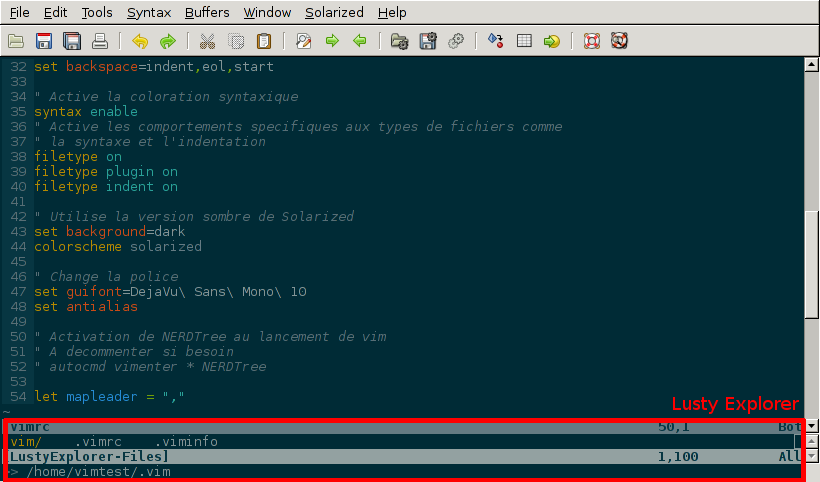
\includegraphics[width=\linewidth]{vim-lusty.png}
  \caption{\vim avec Lusty Explorer d'activé en bas.}
  \label{fig:vim-lusty}
\end{figure}

Je vous conseille maintenant de désactiver \emph{The Nerd Tree} (en commentant la ligne au dessus du \emph{mapleader} comme je l'ai fait dans la figure \ref{fig:vim-lusty-fuzzy}), il ne vous servira plus à grand chose, \emph{Lusty Explorer} le remplace à merveille.

Vous pouvez constater sur la figure \ref{fig:vim-lusty} qu'il y a deux parties à \emph{Lusty Explorer}. La partie basse vous indique le répertoire que vous êtes en train d'explorer et la partie haute liste le contenu de ce répertoire. En surbrillance se trouve l'élément couramment sélectionné. Dans le cas de la figure \ref{fig:vim-lusty} c'est le répertoire \Verb|.vim/| en jaune  (la couleur pourra être différente en fonction de votre thème).

\emph{Lusty Explorer} utilise une fonctionnalité de \emph{Fuzzy matching} qui va vous permettre de ne taper qu'une partie d'un nom de fichier pour le sélectionner. Dans mon exemple, si, dans la fenêtre de \emph{Lusty}, je saisi \Verb|.vimi| il va me sélectionner le fichier \Verb|.viminfo| sans que j'ai à lui spécifier le nom entier, je n'aurais ensuite plus qu'à appuyer sur \ttenter pour ouvrir le fichier dans \vim. La figure \ref{fig:vim-lusty-fuzzy} vous montre l'exemple en question.

\begin{figure}%
  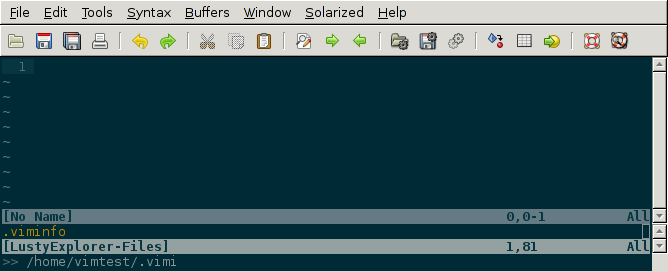
\includegraphics[width=\linewidth]{vim-lusty-fuzzy.png}
  \caption{Lusty Explorer et le Fuzzy matching.}
  \label{fig:vim-lusty-fuzzy}
\end{figure}

\emph{Lusty Explorer} dispose en plus de quelques raccourcis bien pratiques pour utiliser le navigateur de fichiers :

\begin{itemize}
    \item \tctrl + \tn\xspace pour sélectionner le fichier/répertoire suivant
    \item \tctrl + \tp pour sélectionner le fichier/répertoire précédent
    \item \tctrl + \tw pour descendre au répertoire parent
    \item \tctrl + \te crée un nouveau fichier vide (non sauvegardé sur le disque) avec le nom spécifié actuellement dans \emph{Lusty Explorer}. Vous n'aurez plus qu'à utiliser \vimcmd{:w} pour écrire le contenu du fichier sur le disque.
\end{itemize}

\emph{Lusty Explorer} s'utilise donc pour deux choses : naviguer sur votre système de fichiers avec \vimshortcut{,lr} et \vimshortcut{,lf}, et naviguer entre vos fichiers ouverts (buffers) avec \vimshortcut{'lb}. Personnellement j'utilise moins la recherche dans les buffers avec \vimshortcut{,lg}, à vous de tester et de vous faire votre propre opinion.

Je vous conseille en guise de test d'ouvrir plusieurs fichiers avec \vimshortcut{,lr} ou \vimshortcut{,lf}. Ensuite, entraînez-vous à naviguer entre ces différents fichiers ouverts en même temps à l'aide de \vimshortcut{,lb}. C'est une des combinaisons que j'utilise le plus au quotidien.

Ce plugin est indispensable et ajoute à lui seul énormément de valeur à \vim : se passer de la souris pour ouvrir des fichiers. Prenez donc le temps nécessaire pour l'apprendre correctement, c'est un investissement qui vaut le coup.

\section{Recherche dans les fichiers sur le disque : \emph{Ack}}

Lorsque l'on édite un fichier appartenant à un projet plus gros contenant lui même beaucoup de fichiers, il arrive souvent de vouloir rechercher une occurrence d'une chaîne de caractères dans tous les fichiers du projet. Pour ce faire, \vim dispose d'un plugin permettant d'utiliser \emph{Ack} pour faire cette recherche.

\emph{Ack}\sidenote{\url{http://betterthangrep.com/}} est un programme écrit en \emph{perl} qui remplace avantageusement le bon vieux \emph{grep} pour effectuer des recherches dans des fichiers. Il a en revanche un désavantage par rapport à \emph{grep} : il est rarement installé par défaut. Nous allons donc commencer par installer \emph{Ack} avant de pouvoir aller plus loin. Cela va bien sûr dépendre de la plateforme sur laquelle vous utilisez \vim, vous pourrez trouver différentes instructions en fonction de votre plateforme sur la page du plugin : \url{http://github.com/mileszs/ack.vim#installation}.

Pour Debian/Ubuntu : \textbf{\emph{sudo apt-get install ack-grep}}. Pour Mac Os X vous allez avoir besoin de Homebrew (\url{http://mxcl.github.com/homebrew/}) en utilisant \textbf{\emph{brew install ack}}. Pour les utilisateurs de MacPorts ça sera avec la commande \textbf{\emph{sudo port install p5-app-ack}}. Pour Windows installez Strawberry Perl (\url{http://strawberryperl.com/}) et dans le shell de commandes exécutez \textbf{\emph{C:\textbackslash>cpan App::Ack}}. Vous devriez ensuite pouvoir utiliser la commande \textbf{ack} dans votre terminale de commandes en lieu et place de \textbf{grep}.

Rendez-vous sur la page du plugin ack\sidenote{\url{http://www.vim.org/scripts/script.php?script\_id=2572}} et téléchargez la dernière version (à l'heure où j'écris ces lignes c'est la version 0.3.1). Décompressez l'archive dan votre répertoire \Verb|~/.vim/bundle/|, de manière à obtenir une structure de ce type :

\begin{verbatim}

bundle
|-- ack
|   |-- doc
|   |   `-- ack.txt
|   `-- plugin
|       `-- ack.vim
…
\end{verbatim}

Comme d'habitude assurez-vous que vos modifications sont bien prises en compte en redémarrant \vim ou en tapant \vimcmd{:source \~{}/.vimrc} en mode normal.

Il va ensuite falloir ajouter quelques lignes à notre fichier \vimrc pour faciliter d'utilisation du plugin :

\begin{listing}[H]

    \begin{minted}[bgcolor=bg, gobble=8]{vim}
        " Parametres par defaut pour ack
        let g:ackprg="ack -H --nocolor --nogroup --column"
        " Place un marqueur et cherche
        nmap <leader>j mA:Ack<space>
        " Place un marqueur et cherche le mot sous le curseur
        nmap <leader>ja mA:Ack "<C-r>=expand("<cword>")<cr>"
        nmap <leader>jA mA:Ack "<C-r>=expand("<cWORD>")<cr>"
    \end{minted}
    \caption{Configuration du plugin Ack.}
    \label{code:leader}
\end{listing}

Ack recherchera alors à partir du répertoire où se trouve votre fichier couramment ouvert. Il vous affichera les résultats dans une fenêtre que l'on appelle \emph{Quickfix Window}. \TODO faire un screen


Voici quelques commandes disponibles dans cette fenêtre :

\begin{itemize}
    \item \textbf{o} : ouvrir (idem que <Entrée>
    \item \textbf{go} : voir un aperçu (ouvre le fichier mais mantient le focus sur les résultats de ack.vim)
    \item \textbf{t} : ouvrir dans un nouvel onglet
    \item \textbf{T} : ouvrir dans un nouvel onglet en arrière plan
    \item \textbf{h} : ouvrir en séparant la fenêtre horizontalement
    \item \textbf{v} : ouvrir en séparant la fenètre verticalement
    \item \textbf{q} : fermer la fenêtre quickfix
\end{itemize}

\section{Recherche de fichiers sur le disque}

Utile pour de grands projets avec beaucoup de fichiers

ctrlp : \url{https://github.com/kien/ctrlp.vim}

\section{Complétion automatique}

neocomplcache : \url{http://www.vim.org/scripts/script.php?script\_id=2620}

\section{Les plugins avancés}

surround : \url{http://www.vim.org/scripts/script.php?script\_id=1697}

fugitive : git management \url{https://github.com/tpope/vim-fugitive}

syntastic : checking code syntax \url{https://github.com/scrooloose/syntastic}

ctags + ctrlp : code navigation \url{http://andrew-stewart.ca/2012/10/31/vim-ctags}


\chapter{Pense-bête et exemples}

Nous venons de faire un tour d'horizon de tout ce qui est nécessaire pour bien commencer dans la vie avec \vim. Tout cela devrait être suffisant pour pouvoir l'utiliser au quotidien. C'est le secret de la réussite avec \vim : réussir à l'encrer dans nos habitudes journalières. Une fois que cela est fait, le reste devrait couler de source.

Cette dernière partie est là pour vous donner un endroit de référence où vous pourrez revenir comme bon vous semble lorsque vous serez un peu perdu sur comment faire telle ou telle chose avec \vim. Ce chapitre est composé de deux parties. La première est un ensemble de questions réponses qui couvre les principaux problèmes que les débutants rencontrent lorsqu'ils commencent. Le but est de répondre aux questions du type : « rha mais comment on fait ça, c'était pourtant si simple avec mon ancien éditeur ». La seconde partie est une liste (non exhaustive) des commandes \vim les plus utiles dont vous pourrez vous servir comme pense-bête. Allez hop, au boulot.

\section{Questions / réponses}

\subsection{Comment quitter \vim ?}

La première chose à faire est de se mettre en mode normal. Grosso modo, excitez-vous sur \ttesc ou \ttsemicolon en fonction de votre configuration et vous devriez vous retrouver en mode normal. Ensuite tapez \vimcmd{:q} pour quitter. Il y a de grandes chances que \vim ne vous laisse pas faire. Si vous avez des modifications non enregistrées par exemple, il ne voudra pas quitter. Vous pouvez annuler les modification en le forçant à quitter grâce à l'utilisation de \vimcmd{!} comme ceci : \vimcmd{:q!}. Vous pouvez aussi enregistrer vos modifications puis quitter comme ceci : \vimcmd{:wq}.

\subsection{Comment sauvegarder sous ?}

En mode normal, si vous tapez \vimcmd{:w}, \vim par défaut sauvegarde vos modifications dans le fichier courant. Si vous souhaitez utiliser un autre nom de fichier pour « sauvegarder sous », vous avez juste à lui spécifier le nom du fichier après \vimcmd{w} comme ceci : \vimcmd{:w monfichier.txt}. \vim sauvegardera alors votre fichier sous le nom \emph{monfichier.txt}. En revanche \vim n'ouvrira pas \emph{monfichier.txt}, il restera sur votre précédent fichier.

Si vous souhaitez que \vim sauvegarde sous \emph{monfichier.txt} et ouvre ensuite ce fichier dans le tampon courant, vous devrez utiliser \vimcmd{:sav monfichier.txt}.

\subsection{Comment copier/couper coller ?}

Celle là est facile, j'y ai déjà consacré un chapitre, cf. \nameref{sec:se-deplacer}. 

En résumé :

\begin{itemize}
    \item Passez en mode visuel avec \ttv,
    \item Sélectionnez ce que vous voulez copier en vous déplaçant,
    \item Copiez avec \tty\xspace ou couper avec \ttx ou \ttd,
    \item Collez après l'emplacement du curseur avec \ttp ou avant l'emplacement du curseur avec \ttP.
\end{itemize}

\subsection{Comment créer un nouveau fichier ?}

La façon traditionnelle de faire est de taper, en mode normal, \vimcmd{:e monfichier.txt} pour ouvrir un tampon (buffer) vide. Ensuite, sauvegardez votre tampon grâce à \vimcmd{:w}. Il sera sauvegardé sous le nom \Verb|monfichier.txt| dans le répertoire courant.

Vous pouvez aussi utiliser Lusty Explorer (cf. \nameref{lusty}) pour ce faire. Lancez le grâce à \vimcmd{,lr} ou \vimcmd{,lf}, tapez le nom du fichier que vous souhaitez créer puis appuyez sur \ttctrl puis en même temps \tte. Vous pouvez ensuite le sauvegarder de la même manière que ci-dessus.

\subsection{Annuler / Refaire}

Pour annuler il suffit d'utiliser \ttu en mode normal. Pour annuler le annuler (donc refaire) maintenez \ttctrl appuyée puis \ttr.

\section{Pense-bête}

\section{Fichiers}

\begin{tabularx}{17cm}{|X|c|X|}
  \hline
  Résultat attendu & Action & Commentaire \\
  \hline \hline
  \textbf{Sauvegarder} & \vimcmd{:w} & (w pour write)\\
  \hline
  \textbf{Sauvegarder sous} & \vimcmd{:w \emph{nomdefichier.txt}} & Sauvegarde sous nomdefichier.txt mais n'ouvre pas nomdefichier.txt \\
  \hline
  \textbf{Sauvegarder sous / ouvre} & \vimcmd{:sav \emph{nomdefichier.txt}} & Sauvegarde sous et ouvre nomdefichier.txt  \\
  \hline
  \textbf{Quitter sans sauvegarder (forcer à quitter)} & \vimcmd{:q!} & \\
  \hline
  \textbf{Sauvegarder et quitter} & \vimcmd{:wq} (wq pour write and quit) & \\
  \hline
\end{tabularx}

\section{Déplacements}

\begin{tabularx}{17cm}{|X|c|}
  \hline
  Résultat attendu & Action \\
  \hline \hline
  \textbf{Se déplacer d'un caractère à gauche} & \vimcmd{h} \\
  \hline
  \textbf{Se déplacer d'un caractère en bas} & \vimcmd{j} \\
  \hline
  \textbf{Se déplacer d'un caractère en haut} & \vimcmd{k} \\
  \hline
  \textbf{Se déplacer d'un caractère à droite} & \vimcmd{l} \\
  \hline
  \textbf{Se déplacer à la fin d'un mot} & \vimcmd{e} \\
  \hline
  \textbf{Se déplacer au début d'un mot} & \vimcmd{b} \\
  \hline
  \textbf{Se déplacer au début du mot suivant} & \vimcmd{w} \\
  \hline
  \textbf{Se déplacer à la ligne 42} & \vimcmd{:42} \\
  \hline
  \textbf{Se déplacer au début du fichier} & \vimcmd{gg} ou \vimcmd{:0} \\
  \hline
  \textbf{Se déplacer à la fin du fichier} & \vimcmd{GG} ou \vimcmd{:\$} \\
  \hline
  \textbf{Se déplacer à la fin de la ligne} & \vimcmd{\$} \\
  \hline
  \textbf{Se déplacer au premier caractère non vide de la ligne} & \vimcmd{\^{ }} \\
  \hline
  \textbf{Se déplacer au début de la ligne} & \vimcmd{0} \\
  \hline
  \textbf{Descendre d'une page} & \vimcmd{Ctrl+f} \\
  \hline
  \textbf{Monter d'une page} & \vimcmd{Ctrl+b} \\
  \hline
  \textbf{Se déplacer à la première ligne de l'écran} & \vimcmd{H} \\
  \hline
  \textbf{Se déplacer au milieu de l'écran} & \vimcmd{M} \\
  \hline
  \textbf{Se déplacer à la dernière ligne de l'écran} & \vimcmd{L} \\
  \hline
\end{tabularx}

\section{Édition de texte}

\begin{tabularx}{17cm}{|X|c|X|}
  \hline
  Résultat attendu & Action & Commentaire \\
  \hline \hline
  \textbf{Insérer avant le curseur} & \vimcmd{i} & \\
  \hline
  \textbf{Insérer avant le premier caractère non vide de la ligne} & \vimcmd{I} & \\
  \hline
  \textbf{Insérer après le curseur} & \vimcmd{a} & \\
  \hline
  \textbf{Insérer à la fin de la ligne} & \vimcmd{A} & \\
  \hline
  \textbf{Insérer une nouvelle ligne en dessous} & \vimcmd{o} & \\
  \hline
  \textbf{Insérer une nouvelle ligne au dessus} & \vimcmd{O} & \\
  \hline
  \textbf{Remplace le reste de la ligne} & \vimcmd{C} & \\
  \hline
  \textbf{Remplace un seul caractère (et reste en mode normal)} & \vimcmd{r} & \\
  \hline
  \textbf{Supprime le caractère après le curseur (comme la touche suppr.)} & \vimcmd{x} & \\
  \hline
  \textbf{Supprime le caractère avant le curseur (comme la touche backspace)} & \vimcmd{X} & \\
  \hline
  \textbf{Supprime la ligne courante} & \vimcmd{dd} & \\
  \hline
  \textbf{Copie la ligne courante} & \vimcmd{yy} & \\
  \hline
  \textbf{Colle après le curseur. Si c'est une ligne, colle la ligne en dessous.} & \vimcmd{p} & \\
  \hline
  \textbf{Colle avant le curseur. Si c'est une ligne, colle la ligne au dessus.} & \vimcmd{P} & \\
  \hline
  \textbf{Intervertit la case des caractères (majuscules / minuscules)} & \vimcmd{\textasciitilde} & Marche en mode visuel\\
  \hline
  \textbf{Déplace le texte vers la droite (indentation)} & \vimcmd{>} & Marche en mode visuel \\
  \hline
  \textbf{Déplace le texte vers la gauche} & \vimcmd{<} & Marche en mode visuel \\
  \hline
  \textbf{En mode visuel, supprime la sélection} & \vimcmd{d} & Mode visuel \\
  \hline
  \textbf{En mode visuel, remplace la sélection} & \vimcmd{c} & Mode visuel \\
  \hline
  \textbf{En mode visuel, copie la sélection} & \vimcmd{y} & Mode visuel \\
  \hline
  \textbf{Annuler (Undo)} & \vimcmd{u} & \\
  \hline
  \textbf{Refaire (Redo)} & \vimcmd{Ctrl+r} & \\
  \hline
\end{tabularx}

\section{Chercher et/ou remplacer}

\bigskip



\listoffigures

\printindex

\end{document}

